\documentclass[a4paper,12pt]{article}
\usepackage{amsmath}
\usepackage{amssymb,amsthm,graphicx}
\usepackage{enumitem}
\usepackage{color}
\usepackage{epsfig}
\usepackage{graphics}
\usepackage{pdfpages}
\usepackage{subcaption}
\usepackage[font=small]{caption}
\usepackage[hang,flushmargin]{footmisc} 
\usepackage{placeins}
\usepackage{diagbox}
\usepackage{float}
\usepackage{rotating,tabularx}
\usepackage{booktabs}
\usepackage[mathscr]{euscript}
\usepackage{natbib}
\usepackage{setspace}
\usepackage{mathrsfs}
\usepackage[left=2.7cm,right=2.7cm,bottom=2.7cm,top=2.7cm]{geometry}
\parindent0pt 


% General

\newcommand{\reals}{\mathbb{R}}
\newcommand{\integers}{\mathbb{Z}}
\newcommand{\naturals}{\mathbb{N}}

\newcommand{\pr}{\mathbb{P}}        % probability
\newcommand{\ex}{\mathbb{E}}        % expectation
\newcommand{\var}{\textnormal{Var}} % variance
\newcommand{\cov}{\textnormal{Cov}} % covariance

\newcommand{\law}{\mathcal{L}} % law of X
\newcommand{\normal}{N}        % normal distribution 

\newcommand{\argmax}{\textnormal{argmax}}
\newcommand{\argmin}{\textnormal{argmin}}

\newcommand{\ind}{\mathbbm{1}} % indicator function
\newcommand{\kernel}{K} % kernel function
\newcommand{\wght}{W} % kernel weight
\newcommand{\thres}{\pi} % threshold parameter


% Convergence

\newcommand{\convd}{\stackrel{d}{\longrightarrow}}              % convergence in distribution
\newcommand{\convp}{\stackrel{P}{\longrightarrow}}              % convergence in probability
\newcommand{\convas}{\stackrel{\textrm{a.s.}}{\longrightarrow}} % convergence almost surely
\newcommand{\convw}{\rightsquigarrow}                           % weak convergence


% Theorem-like declarations

\theoremstyle{plain}

\newtheorem{theorem}{Theorem}[section]
\newtheorem{prop}[theorem]{Proposition}
\newtheorem{lemma}[theorem]{Lemma}
\newtheorem{corollary}[theorem]{Corollary}
\newtheorem*{theo}{Theorem}
\newtheorem{propA}{Proposition}[section]
\newtheorem{lemmaA}[propA]{Lemma}
\newtheorem{definition}{Definition}[section]
\newtheorem{remark}{Remark}[section]
\renewcommand{\thelemmaA}{A.\arabic{lemmaA}}
\renewcommand{\thepropA}{A.\arabic{propA}}
\newtheorem*{algo}{Clustering Algorithm}


% Theorem numbering to the left

\makeatletter
\newcommand{\lefteqno}{\let\veqno\@@leqno}
\makeatother


% Heading

\newcommand{\heading}[2]
{  \setcounter{page}{1}
   \begin{center}

   \phantom{Distance to upper boundary}
   \vspace{0.5cm}

   {\LARGE \textbf{#1}}
   \vspace{0.4cm}
 
   {\LARGE \textbf{#2}}
   \end{center}
}


% Authors

\newcommand{\authors}[4]
{  \parindent0pt
   \begin{center}
      \begin{minipage}[c][2cm][c]{5cm}
      \begin{center} 
      {\large #1} 
      \vspace{0.05cm}
      
      #2 
      \end{center}
      \end{minipage}
      \begin{minipage}[c][2cm][c]{5cm}
      \begin{center} 
      {\large #3}
      \vspace{0.05cm}

      #4 
      \end{center}
      \end{minipage}
   \end{center}
}

%\newcommand{\authors}[2]
%{  \parindent0pt
%   \begin{center}
%   {\large #1} 
%   \vspace{0.1cm}
%      
%   #2 
%   \end{center}  
%}


% Version

\newcommand{\version}[1]
{  \begin{center}
   {\large #1}
   \end{center}
   \vspace{3pt}
} 










\begin{document}



\heading{Multiscale Inference}{and Long-Run Variance Estimation}{in Nonparametric Regression}{with Time Series Errors}

%\vspace{-0.5cm}

\authors{Marina Khismatullina\renewcommand{\thefootnote}{1}\footnotemark[1]}{University of Bonn}{Michael Vogt\renewcommand{\thefootnote}{2}\footnotemark[2]}{University of Bonn} 
\footnotetext[1]{Address: Bonn Graduate School of Economics, University of Bonn, 53113 Bonn, Germany. Email: \texttt{marina.k@uni-bonn.de}.}
\renewcommand{\thefootnote}{2}
\footnotetext[2]{Corresponding author. Address: Department of Economics and Hausdorff Center for Mathematics, University of Bonn, 53113 Bonn, Germany. Email: \texttt{michael.vogt@uni-bonn.de}.}
\renewcommand{\thefootnote}{\arabic{footnote}}
\setcounter{footnote}{2}

\vspace{-0.5cm}

\version{\today}

\vspace{-1.2cm}



\renewcommand{\abstractname}{}
\begin{abstract}
\noindent In this paper, we develop new multiscale methods to test qualitative hypotheses about the function $m$ in the nonparametric regression model $Y_{t,T} = m(t/T) + \varepsilon_t$ with time series errors $\varepsilon_t$. In time series applications, $m$ represents a nonparametric time trend. Practitioners are often interested in whether the trend $m$ has certain shape properties. For example, they would like to know whether $m$ is constant or whether it is increasing/decreasing in certain time \textcolor{red}{intervals}. Our multiscale methods allow to test for such shape properties of the trend $m$. In order to perform the methods, we require an estimator of the long-run error variance $\sigma^2 = \sum\nolimits_{\ell=-\infty}^{\infty} \cov(\varepsilon_0,\varepsilon_{\ell})$. \textcolor{red}{We propose a new difference-based estimator of $\sigma^2$ for the case that $\{ \varepsilon_t \}$ belongs to the class of AR($\infty$) processes.} In the technical part of the paper, we derive asymptotic theory for the proposed multiscale test and the estimator of the long-run error variance. The theory is complemented by a simulation study and an empirical application to climate data. 
\end{abstract}


\renewcommand{\baselinestretch}{1.2}\normalsize

\textbf{Key words:} Multiscale statistics; long-run variance; nonparametric regression; time series errors; shape constraints; strong approximations; anti-concentration bounds.

\textbf{AMS 2010 subject classifications:} 62E20; 62G10; 62G20; 62M10. 

\numberwithin{equation}{section}
\allowdisplaybreaks[4]




\section{Introduction}\label{sec-intro}


The analysis of time trends is an important aspect of many time series applications. In a wide range of situations, practitioners are particularly interested in certain shape properties of the trend. They raise questions such as the following: Does the observed time series have a trend at all? If so, is the trend increasing/decreasing in certain time regions? Can one identify the regions of increase/decrease? As an example, consider the time series plotted in Figure \ref{temp_data} which shows the yearly mean temperature in Central England from 1659 to 2017. Climatologists are very much interested in learning about the trending behaviour of temperature time series like this; see e.g.\ \cite{Benner1999} and \cite{Rahmstorf2017}. Among other things, they would like to know whether there is an upward trend in the Central England mean temperature towards the end of the sample as visual inspection might suggest.


\begin{figure}
\centering
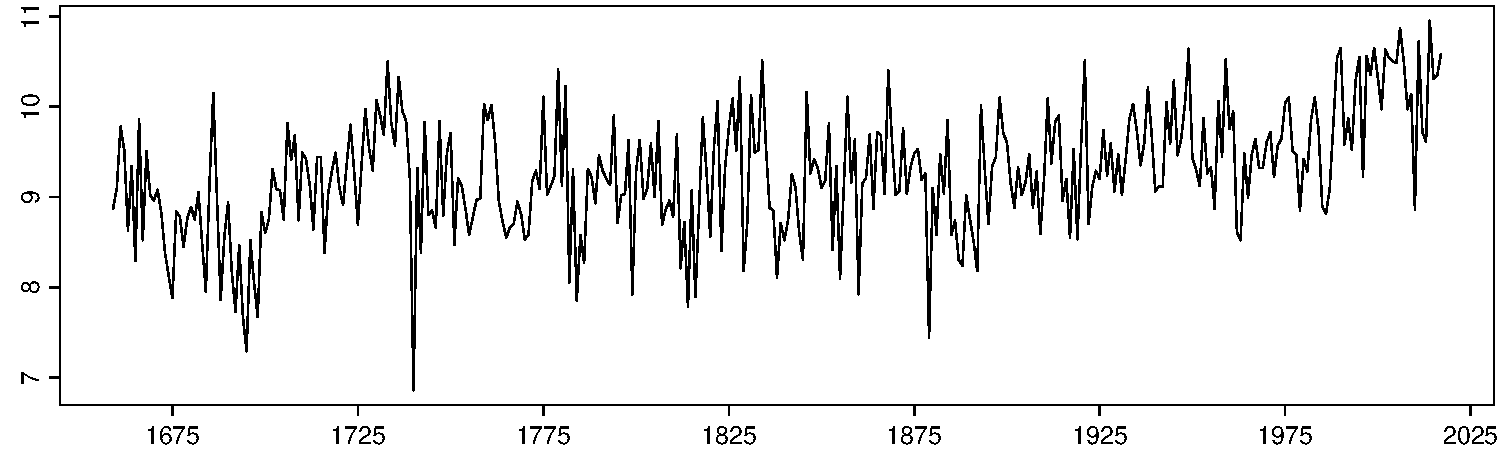
\includegraphics[width=0.9\textwidth]{Plots/temp_data.pdf}
\vspace{0.15cm}

\caption{Yearly mean temperature in Central England from 1659 to 2017 measured in $^\circ$C.}\label{temp_data}
\end{figure}


In this paper, we develop new methods to test for certain shape properties of a nonparametric time trend. We in particular construct a multiscale test which allows to identify local increases/decreases of the trend function. 
%We in particular construct a multiscale test for local increases/de\-creases of the trend function. The proposed test allows to identify, with a pre-specified statistical confidence, time regions where there is an increase/decrease in the trend. 
%identify subintervals on which the function $m$ deviates significantly from the null hypothesis of constancy. 
We develop our test in the context of the following model setting: We observe a time series $\{ Y_{t,T}: 1 \le t \le T \}$ of the form 
\begin{equation}\label{model-intro}
Y_{t,T} = m \Big( \frac{t}{T} \Big) + \varepsilon_t
\end{equation}
for $1 \le t \le T$, where $m: [0,1] \rightarrow \mathbb{R}$ is an unknown nonparametric regression function and the error terms $\varepsilon_t$ form a stationary time series process with $\ex[\varepsilon_t] = 0$. In a time series context, the design points $t/T$ represent the time points of observation and $m$ is a nonparametric time trend. As usual in nonparametric regression, we let the function $m$ depend on rescaled time $t/T$ rather than on real time $t$. A detailed description of model \eqref{model-intro} is provided in Section \ref{sec-model}.


Our multiscale test is developed step by step in Section \ref{sec-method}. Roughly speaking, the procedure can be outlined as follows: Let $H_0(u,h)$ be the hypothesis that $m$ is constant in the time window $[u-h,u+h] \subseteq [0,1]$, where $u$ is the midpoint and $2h$ the size of the window. In a first step, we set up a test statistic $\widehat{s}_T(u,h)$ for the hypothesis $H_0(u,h)$. In a second step, we aggregate the statistics $\widehat{s}_T(u,h)$ for a large number of different time windows $[u-h,u+h]$. We thereby construct a multiscale statistic which allows to test the hypothesis $H_0(u,h)$ simultaneously for many time windows $[u-h,u+h]$. In the technical part of the paper, we derive the theoretical properties of the resulting multiscale test. To do so, we come up with a proof strategy which combines strong approximation results for dependent processes with anti-concentration bounds for Gaussian random vectors. This strategy is of interest in itself and may be applied to other multiscale test problems for dependent data. As shown by our theoretical analysis, our multiscale test is a rigorous level-$\alpha$-test of the overall null hypothesis $H_0$ that $H_0(u,h)$ is simultaneously fulfilled for all time windows $[u-h,u+h]$ under consideration. Moreover, for a given significance level $\alpha \in (0,1)$, the test allows to make simultaneous confidence statements of the following form: We can claim, with statistical confidence $1-\alpha$, that there is an increase/decrease in the trend $m$ on all time windows $[u-h,u+h]$ for which the hypothesis $H_0(u,h)$ is rejected. Hence, the test allows to identify, with a pre-specified statistical confidence, time regions where the trend $m$ is increasing/decreasing. 


For independent data, multiscale tests have been developed in a variety of different contexts in recent years. In the regression context, \cite{ChaudhuriMarron1999,ChaudhuriMarron2000} introduced the so-called SiZer method which has been extended in various directions; see e.g.\ \cite{HannigMarron2006} where a refined distribution theory for SiZer is derived. \cite{HallHeckman2000} constructed a multiscale test on monotonicity of a regression function. \cite{DuembgenSpokoiny2001} developed a multiscale approach which works with additively corrected supremum statistics and derived theoretical results in the context of a continuous Gaussian white noise model. Rank-based multiscale tests for nonparametric regression were proposed in \cite{Duembgen2002} and \cite{Rohde2008}. More recently, \cite{ProkschWernerMunk2018} have constructed multiscale tests for inverse regression models. In the context of density estimation, multiscale tests have been investigated in \cite{DuembgenWalther2008}, \cite{RufibachWalther2010}, \cite{SchmidtHieber2013} and \cite{EckleBissantzDette2017} among others. 


Whereas a large number of multiscale tests for independent data have been developed in recent years, multiscale tests for dependent data are much rarer. Most notably, there are some extensions of the SiZer approach to a time series context. \cite{Rondonotti2004} and \cite{Rondonotti2007} have introduced SiZer methods for dependent data which can be used to find local increases/decreases of a trend and which may thus be regarded as an alternative to our multiscale test. However, these SiZer methods are mainly designed for data exploration rather than for rigorous statistical inference. Our multiscale method, in contrast, is a rigorous level-$\alpha$-test of the hypo\-thesis $H_0$ which allows to make simultaneous confidence statements about the time regions where the trend $m$ is increasing/decreasing. Some theoretical results for dependent SiZer methods have been derived in \cite{ParkHannigKang2009}, but only under a quite severe restriction: Only time windows $[u-h,u+h]$ with window sizes or scales $h$ are taken into account that remain bounded away from zero as the sample size $T$ grows. Scales $h$ that converge to zero as $T$ increases are excluded. This effectively means that only large time windows $[u-h,u+h]$ are taken into consideration. Our theory, in contrast, allows to simultaneously consider scales $h$ of fixed size and scales $h$ that converge to zero at various different rates. We are thus able to take into account time windows of many different sizes. \textcolor{red}{In Section \ref{subsec-method-comparison}, we compare our approach to SiZer methods in more detail.}


Our multiscale approach is also related to Wavelet-based methods: Similar to the latter, it takes into account different locations $u$ and resolution levels or scales $h$ simultaneously. However, while our multiscale approach is designed to test for local increases/decreases of a nonparametric trend, Wavelet methods are commonly used for other purposes. Among other things, they are employed for estimating/reconstructing nonparametric regression curves [see e.g.\ \cite{Donoho1995} or \cite{vonSachsMacGibbon2000}] and for change point detection [see e.g.\ \citet{ChoFryzlewicz2012}]. 


%Whereas a large number of multiscale tests for independent data have been developed in recent years, multiscale tests for dependent data are much rarer. Most notably, there are some extensions of the SiZer approach to a time series context. \cite{Rondonotti2004}, \cite{Rondonotti2007} and \cite{ParkHannigKang2009} have developed SiZer methods for dependent data which can be regarded as an alternative to our multiscale test. However, these SiZer methods are mainly designed for data exploration rather than rigorous statistical inference. Our multiscale method, in contrast, is a rigorous level-$\alpha$-test of the hypo\-thesis $H_0$, which is backed up by a complete asymptotic theory. Moreover, it allows to make simultaneous confidence statements about the time regions where the trend function $m$ is increasing/decreasing, which is not possible with the SiZer tools of \cite{Rondonotti2004}, \cite{Rondonotti2007} and \cite{ParkHannigKang2009}. Our multiscale approach is also related to Wavelet-based methods: It investigates the data on different intervals $[u-h,u+h]$. Similar to Wavelet-based procedures, it thus takes into account different locations $u$ and resolution levels $h$ simultaneously. Nevertheless, we are not aware of any Wavelet-based test for local increases/decreases of the nonparametric trend function in model \eqref{model-intro}. Wavelet methods have been used for other purposes in the literature such as estimating/reconstructing nonparametric regression functions [see e.g.\ \cite{Donoho1995} or \cite{vonSachsMacGibbon2000}] and change point detection [see e.g.\ \citet{ChoFryzlewicz2012}]. 


The test statistic of our multiscale method depends on the long-run error variance $\sigma^2 = \sum\nolimits_{\ell=-\infty}^{\infty} \cov(\varepsilon_0,\varepsilon_{\ell})$, which is usually unknown in practice. To carry out our multiscale test, we thus require an estimator of $\sigma^2$. Indeed, such an estimator is required for virtually all inferential procedures in the context of model \eqref{model-intro}. Hence, the problem of estimating $\sigma^2$ in model \eqref{model-intro} is of broader interest and has received a lot of attention in the literature; see \cite{MuellerStadtmueller1988}, \cite{Herrmann1992} and \cite{Hall2003} among many others. In Section \ref{sec-error-var}, 
%we discuss several estimators of $\sigma^2$ which are valid under different conditions on the error process $\{\varepsilon_t\}$. 
\textcolor{red}{we introduce a new difference-based estimator of $\sigma^2$ for the case that $\{ \varepsilon_t \}$ belongs to the class of AR($\infty$) processes}. This estimator improves on existing methods in several respects. 


The methodological and theoretical analysis of the paper is complemented by a simulation study in Section \ref{sec-sim} and an empirical application in Section \ref{sec-data}. In the simulation study, we examine the finite sample properties of our multiscale test and compare it to the dependent SiZer methods introduced in \cite{Rondonotti2004} and \cite{Rondonotti2007}. Moreover, we investigate the small sample performance of our estimator of $\sigma^2$ in the AR($p$) case and compare it to the estimator of \cite{Hall2003}. In Section \ref{sec-data}, we use our methods to analyse the temperature data from Figure \ref{temp_data} \textcolor{red}{as well as a sample of global temperature data}. 




\section{The model}\label{sec-model}


We now describe the model setting in detail which was briefly outlined in the Introduction. We observe a time series $\{Y_{t,T}: 1 \le t \le T \}$ of length $T$ which satisfies the nonparametric regression equation 
\begin{equation}\label{model}
Y_{t,T} = m \Big( \frac{t}{T} \Big) + \varepsilon_t 
\end{equation}
for $1 \le t \le T$. Here, $m$ is an unknown nonparametric function defined on $[0,1]$ and $\{ \varepsilon_t: 1 \le t \le T \}$ is a zero-mean stationary error process. For simplicity, we restrict attention to equidistant design points $x_t = t/T$. However, our methods and theory can also be carried over to non-equidistant designs. The stationary error process $\{\varepsilon_t\}$ is assumed to have the following properties: 
\begin{enumerate}[label=(C\arabic*),leftmargin=1.05cm]

\item \label{C-err1} The variables $\varepsilon_t$ allow for the representation $\varepsilon_t = G(\ldots,\eta_{t-1},\eta_t,\eta_{t+1},\ldots)$, where $\eta_t$ are i.i.d.\ random variables and $G: \reals^\integers \rightarrow \reals$ is a measurable function. 

\item \label{C-err2} It holds that $\| \varepsilon_t \|_q < \infty$ for some $q > 4$, where $\| \varepsilon_t \|_q = (\ex|\varepsilon_t|^q)^{1/q}$. 

\end{enumerate}
Following \cite{Wu2005}, we impose conditions on the dependence structure of the error process $\{\varepsilon_t\}$ in terms of the physical dependence measure $d_{t,q} = \| \varepsilon_t - \varepsilon_t^\prime \|_q$, where $\varepsilon_t^\prime = G(\ldots,\eta_{-1},\eta_0^\prime,\eta_1,\ldots,\eta_{t-1},\eta_t,\eta_{t+1},\ldots)$ with $\{\eta_t^\prime\}$ being an i.i.d.\ copy of $\{\eta_t\}$. In particular, we assume the following: 
\begin{enumerate}[label=(C\arabic*),leftmargin=1.05cm]
\setcounter{enumi}{2}

\item \label{C-err3} Define $\Theta_{t,q} = \sum\nolimits_{|s| \ge t} d_{s,q}$ for $t \ge 0$. It holds that 
$\Theta_{t,q} = O ( t^{-\tau_q} (\log t)^{-A} )$,  
where $A > \frac{2}{3} (1/q + 1 + \tau_q)$ and $\tau_q = \{q^2 - 4 + (q-2) \sqrt{q^2 + 20q + 4}\} / 8q$. 

\end{enumerate}
The conditions \ref{C-err1}--\ref{C-err3} are fulfilled by a wide range of stationary processes $\{\varepsilon_t\}$. As a first example, consider linear processes of the form $\varepsilon_t = \sum\nolimits_{i=0}^{\infty} c_i \eta_{t-i}$ with $\| \varepsilon_t \|_q < \infty$, where $c_i$ are absolutely summable coefficients and $\eta_t$ are i.i.d.\ innovations with $\ex[\eta_t] = 0$ and $\| \eta_t\|_q < \infty$. Trivially, \ref{C-err1} and \ref{C-err2} are fulfilled in this case. Moreover, if $|c_i| = O(\rho^i)$ for some $\rho \in (0,1)$, then \ref{C-err3} is easily seen to be satisfied as well. As a special case, consider an ARMA process $\{\varepsilon_t\}$ of the form $\varepsilon_t - \sum\nolimits_{i=1}^p a_i \varepsilon_{t-i} = \eta_t + \sum\nolimits_{j=1}^r b_j \eta_{t-j}$  with $\| \varepsilon_t \|_q < \infty$, where $a_1,\ldots,a_p$ and $b_1,\ldots,b_r$ are real-valued parameters. As before, we let $\eta_t$ be i.i.d.\ innovations with $\ex[\eta_t] = 0$ and $\| \eta_t\|_q < \infty$. Moreover, as usual, we suppose that the complex polynomials $A(z) = 1 - \sum\nolimits_{j=1}^p a_jz^j$ and $B(z) = 1 + \sum\nolimits_{j=1}^r b_jz^j$ do not have any roots in common. If $A(z)$ does not have any roots inside the unit disc, then the ARMA process $\{ \varepsilon_t \}$ is stationary and causal. Specifically, it has the representation $\varepsilon_t = \sum\nolimits_{i=0}^{\infty} c_i \eta_{t-i}$ with $|c_i| = O(\rho^i)$ for some $\rho \in (0,1)$, implying that \ref{C-err1}--\ref{C-err3} are fulfilled. The results in \cite{WuShao2004} show that condition \ref{C-err3} (as well as the other two conditions) is not only fulfilled for linear time series processes but also for a variety of non-linear processes. 



\section{The multiscale test}\label{sec-method}


In this section, we introduce our multiscale method to test for local increases/decreases of the trend function $m$ and analyse its theoretical properties. We assume throughout that $m$ is continuously differentiable on $[0,1]$. The test problem under consideration can be formulated as follows: Let $H_0(u,h)$ be the hypothesis that $m$ is constant on the interval $[u-h,u+h]$. Since $m$ is continuously differentiable, $H_0(u,h)$ can be reformulated as
\[ H_0(u,h): m^\prime(w) = 0 \text { for all } w \in [u-h,u+h], \]
where $m^\prime$ is the first derivative of $m$. We want to test the hypothesis $H_0(u,h)$ not only for a single interval $[u-h,u+h]$ but simultaneously for many different intervals. The overall null hypothesis is thus given by
\[ H_0: \text{ The hypothesis } H_0(u,h) \text{ holds true for all } (u,h) \in \mathcal{G}_T, \]
where $\mathcal{G}_T$ is some large set of points $(u,h)$. The details on the set $\mathcal{G}_T$ are discussed at the end of Section \ref{subsec-method-stat} below. Note that $\mathcal{G}_T$ in general depends on the sample size $T$, implying that the null hypothesis $H_0 = H_{0,T}$ depends on $T$ as well. We thus consider a sequence of null hypotheses $\{H_{0,T}: T = 1,2,\ldots \}$ as $T$ increases. For simplicity of notation, we however suppress the dependence of $H_0$ on $T$. In Sections \ref{subsec-method-stat} and \ref{subsec-method-test}, we step by step construct the multiscale test of the hypothesis $H_0$. The theoretical properties of the test are analysed in Section \ref{subsec-method-theo}. 


\subsection{Construction of the multiscale statistic}\label{subsec-method-stat}


We first construct a test statistic for the hypothesis $H_0(u,h)$, where $[u-h,u+h]$ is a given interval. To do so, we consider the kernel average
\begin{equation*}
\widehat{\psi}_T(u,h) = \sum\limits_{t=1}^T w_{t,T}(u,h) Y_{t,T}, 
\end{equation*}
where $w_{t,T}(u,h)$ is a kernel weight and $h$ is the bandwidth. In order to avoid boundary issues, we work with a local linear weighting scheme. We in particular set 
\begin{equation}\label{weights}
w_{t,T}(u,h) = \frac{\Lambda_{t,T}(u,h)}{ \{\sum\nolimits_{t=1}^T \Lambda_{t,T}(u,h)^2 \}^{1/2} }, 
\end{equation}
where
\[ \Lambda_{t,T}(u,h) = K\Big(\frac{\frac{t}{T}-u}{h}\Big) \Big[ S_{T,0}(u,h) \Big(\frac{\frac{t}{T}-u}{h}\Big) - S_{T,1}(u,h) \Big], \]
$S_{T,\ell}(u,h) = (Th)^{-1} \sum\nolimits_{t=1}^T K(\frac{\frac{t}{T}-u}{h}) (\frac{\frac{t}{T}-u}{h})^\ell$ for $\ell = 0,1,2$ and $K$ is a kernel function with the following properties: 
\begin{enumerate}[label=(C\arabic*),leftmargin=1.05cm]
\setcounter{enumi}{3}
\item \label{C-ker} The kernel $K$ is non-negative, symmetric about zero and integrates to one. Moreover, it has compact support $[-1,1]$ and is Lipschitz continuous, that is, $|K(v) - K(w)| \le C |v-w|$ for any $v,w \in \reals$ and some constant $C > 0$. 
\end{enumerate} 
The kernel average $\widehat{\psi}_T(u,h)$ is nothing else than a rescaled local linear estimator of the derivative $m^\prime(u)$ with bandwidth $h$.\footnote{Alternatively to the local linear weights defined in \eqref{weights}, we could also work with the weights $w_{t,T}(u,h) = K^\prime( h^{-1} [u - t/T] )/ \{ \sum\nolimits_{t=1}^T  K^\prime( h^{-1}[u - t/T] )^2 \}^{1/2}$, where the kernel function $K$ is assumed to be differentiable and $K^\prime$ is its derivative. We however prefer to use local linear weights as these have superior theoretical properties at the boundary.}  


A test statistic for the hypothesis $H_0(u,h)$ is given by the normalized kernel average $\widehat{\psi}_T(u,h)/\widehat{\sigma}$, where $\widehat{\sigma}^2$ is an estimator of the long-run variance $\sigma^2 = \sum\nolimits_{\ell=-\infty}^{\infty} \cov(\varepsilon_0,\varepsilon_\ell)$ of the error process $\{\varepsilon_t\}$. The problem of estimating $\sigma^2$ is discussed in detail in Section \ref{sec-error-var}. For the time being, we suppose that $\widehat{\sigma}^2$ is an estimator with reasonable theoretical properties. Specifically, we assume that $\widehat{\sigma}^2 = \sigma^2 + o_p(\rho_T)$ with $\rho_T = o(1/\log T)$. This is a fairly weak condition which is in particular satisfied by the \textcolor{red}{estimator} of $\sigma^2$ analysed in Section \ref{sec-error-var}. The kernel weights $w_{t,T}(u,h)$ are chosen such that in the case of independent errors $\varepsilon_t$, $\var(\widehat{\psi}_T(u,h)) = \sigma^2$ for any location $u$ and bandwidth $h$, where the long-run error variance $\sigma^2$ simplifies to $\sigma^2 = \var(\varepsilon_t)$. In the more general case that the error terms satisfy the weak dependence conditions from Section \ref{sec-model}, $\var(\widehat{\psi}_T(u,h)) = \sigma^2 + o(1)$ for any $u$ and $h$ under consideration. Hence, for sufficiently large sample sizes $T$, the test statistic $\widehat{\psi}_T(u,h)/\widehat{\sigma}$ has approximately unit variance.


We now combine the test statistics $\widehat{\psi}_T(u,h)/\widehat{\sigma}$ for a wide range of different locations $u$ and bandwidths or scales $h$. There are different ways to do so, leading to different types of multiscale statistics. Our multiscale statistic is defined as
\begin{equation}\label{multiscale-stat}
\widehat{\Psi}_T = \max_{(u,h) \in \mathcal{G}_T} \Big\{ \Big|\frac{\widehat{\psi}_T(u,h)}{\widehat{\sigma}}\Big| - \lambda(h) \Big\}, 
\end{equation} 
where $\lambda(h) = \sqrt{2 \log \{ 1/(2h) \}}$ and $\mathcal{G}_T$ is the set of points $(u,h)$ that are taken into consideration. The details on the set $\mathcal{G}_T$ are given below. As can be seen, the statistic $\widehat{\Psi}_T$ does not simply aggregate the individual statistics $\widehat{\psi}_T(u,h)/\widehat{\sigma}$ by taking the supremum over all points $(u,h) \in \mathcal{G}_T$ as in more traditional multiscale approaches. We rather calibrate the statistics $\widehat{\psi}_T(u,h)/\widehat{\sigma}$ that correspond to the bandwidth $h$ by subtracting the additive correction term $\lambda(h)$. This approach was pioneered by \cite{DuembgenSpokoiny2001} and has been used in numerous other studies since then; see e.g.\ \cite{Duembgen2002}, \cite{Rohde2008}, \cite{DuembgenWalther2008}, \cite{RufibachWalther2010}, \cite{SchmidtHieber2013} and \cite{EckleBissantzDette2017}. 
%aggregation scheme has been introduced by ?? and has been used in a variety of other multiscale approaches since then; cp.\ e.g.\ the multiscale tests in ??. 
%We rather follow the approach pioneered by \cite{DuembgenSpokoiny2001} and subtract the additive correction term $\lambda(h)$ from the statistics $\widehat{\psi}_T(u,h)/\widehat{\sigma}$ that correspond to the bandwidth level $h$. 


To see the heuristic idea behind the additive correction $\lambda(h)$, consider for a moment the uncorrected statistic
\begin{equation}\label{multiscale-stat-uncorrected}
\textcolor{red}{\widehat{\Psi}_{T,\text{uncorrected}} = \max_{(u,h) \in \mathcal{G}_T} \Big|\frac{\widehat{\psi}_T(u,h)}{\widehat{\sigma}}\Big|} 
\end{equation}
and suppose that the hypothesis $H_0(u,h)$ is true for all $(u,h) \in \mathcal{G}_T$. For simplicity, assume that the errors $\varepsilon_t$ are i.i.d.\ normally distributed and neglect the estimation error in $\widehat{\sigma}$, that is, set $\widehat{\sigma} = \sigma$. Moreover, suppose that the set $\mathcal{G}_T$ only consists of the points $(u_k,h_\ell) = ((2k - 1)h_\ell,h_\ell)$ with $k = 1,\ldots,\lfloor 1/2h_\ell \rfloor$ and $\ell = 1,\ldots,L$. In this case, we can write
\[ \widehat{\Psi}_{T,\text{uncorrected}} = \max_{1 \le \ell \le L} \max_{1 \le k \le \lfloor 1/2h_\ell \rfloor} \Big|\frac{\widehat{\psi}_T(u_k,h_\ell)}{\sigma}\Big|. \]
Under our simplifying assumptions, the statistics $\widehat{\psi}_T(u_k,h_\ell)/\sigma$ with $k = 1,\ldots,\lfloor 1/2h_\ell \rfloor$ are independent and standard normal for any given bandwidth $h_\ell$. Since the maximum over $\lfloor 1/2h \rfloor$ independent standard normal random variables is $\lambda(h) + o_p(1)$ as $h \rightarrow 0$, we obtain that $\max_{k} \widehat{\psi}_T(u_k,h_\ell)/\sigma$ is approximately of size $\lambda(h_\ell)$ for small bandwidths $h_\ell$. As $\lambda(h) \rightarrow \infty$ for $h \rightarrow 0$, this implies that $\max_{k} \widehat{\psi}_T(u_k,h_\ell)/\sigma$ tends to be much larger in size for small than for large bandwidths $h_\ell$. As a result, the stochastic behaviour of the uncorrected statistic $\widehat{\Psi}_{T,\text{uncorrected}}$ tends to be dominated by the statistics $\widehat{\psi}_T(u_k,h_\ell)$ corresponding to small bandwidths $h_\ell$. The additively corrected statistic $\widehat{\Psi}_T$, in contrast, puts the statistics $\widehat{\psi}_T(u_k,h_\ell)$ corresponding to different bandwidths $h_\ell$ on a more equal footing, thus counteracting the dominance of small bandwidth values. 


The multiscale statistic $\widehat{\Psi}_T$ simultaneously takes into account all locations $u$ and bandwidths $h$ with $(u,h) \in \mathcal{G}_T$. Throughout the paper, we suppose that $\mathcal{G}_T$ is some subset of $\mathcal{G}_T^{\text{full}} = \{ (u,h): u = t/T \text{ for some } 1 \le t \le T \text{ and } h \in [h_{\min},h_{\max}] \}$, where $h_{\min}$ and $h_{\max}$ denote some minimal and maximal bandwidth value, respectively. For our theory to work, we require the following conditions to hold:
\begin{enumerate}[label=(C\arabic*),leftmargin=1.05cm]
\setcounter{enumi}{4}

\item \label{C-grid} $|\mathcal{G}_T| = O(T^\theta)$ for some arbitrarily large but fixed constant $\theta > 0$, where $|\mathcal{G}_T|$ denotes the cardinality of $\mathcal{G}_T$. 

\item \label{C-h} $h_{\min} \gg T^{-(1-\frac{2}{q})} \log T$, that is, $h_{\min} / \{ T^{-(1-\frac{2}{q})} \log T \} \rightarrow \infty$ with $q > 4$ defined in \ref{C-err2} and $h_{\max} < 1/2$.

\end{enumerate}
According to \ref{C-grid}, the number of points $(u,h)$ in $\mathcal{G}_T$ should not grow faster than $T^\theta$ for some arbitrarily large but fixed $\theta > 0$. This is a fairly weak restriction as it allows the set $\mathcal{G}_T$ to be extremely large compared to the sample size $T$. For example, we may work with the set 
\begin{align*}
\mathcal{G}_T = \big\{ & (u,h): u = t/T \text{ for some } 1 \le t \le T \text{ and } h \in [h_{\min},h_{\max}] \\ & \text{ with } h = t/T \text{ for some } 1 \le t \le T  \big\},
\end{align*}
which contains more than enough points $(u,h)$ for most practical applications. Condition \ref{C-h} imposes some restrictions on the minimal and maximal bandwidths $h_{\min}$ and $h_{\max}$. These conditions are fairly weak, allowing us to choose the bandwidth window $[h_{\min},h_{\max}]$ extremely large. The lower bound on $h_{\min}$ depends on the parameter $q$ defined in \ref{C-err2} which specifies the number of existing moments for the error terms $\varepsilon_t$. As one can see, we can choose $h_{\min}$ to be of the order $T^{-1/2}$ for any $q > 4$. Hence, we can let $h_{\min}$ converge to $0$ very quickly even if only the first few moments of the error terms $\varepsilon_t$ exist. If all moments exist (i.e.\ $q = \infty$), $h_{\min}$ may converge to $0$ almost as quickly as $T^{-1} \log T$. Furthermore, the maximal bandwidth $h_{\max}$ is not even required to converge to $0$, which implies that we can pick it very large.


\begin{remark}
The above construction of the multiscale statistic can be easily adapted to hypotheses other than $H_0$. To do so, one simply needs to replace the kernel weights $w_{t,T}(u,h)$ defined in \eqref{weights} by appropriate versions which are suited to test the hypothesis of interest. For example, if one wants to test for local convexity/concavity of $m$, one may define the kernel weights $w_{t,T}(u,h)$ such that the kernel average $\widehat{\psi}_T(u,h)$ is a (rescaled) estimator of the second derivative of $m$ at the location $u$ with bandwidth $h$. 
\end{remark}


\subsection{The test procedure}\label{subsec-method-test}


In order to formulate a test for the null hypothesis $H_0$, we still need to specify a critical value. To do so, we define the statistic
\begin{equation}\label{Phi-statistic}
\Phi_T = \max_{(u,h) \in \mathcal{G}_T} \Big\{ \Big|\frac{\phi_T(u,h)}{\sigma}\Big| - \lambda(h) \Big\},
\end{equation} 
where $\phi_T(u,h) = \sum\nolimits_{t=1}^T w_{t,T}(u,h) \, \sigma Z_t$ and $Z_t$ are independent standard normal random variables. The statistic $\Phi_T$ can be regarded as a Gaussian version of the test statistic $\widehat{\Psi}_T$ under the null hypothesis $H_0$. Let $q_T(\alpha)$ be the $(1-\alpha)$-quantile of $\Phi_T$. Importantly, the quantile $q_T(\alpha)$ can be computed by Monte Carlo simulations and can thus be regarded as known. Our multiscale test of the hypothesis $H_0$ is now defined as follows: For a given significance level $\alpha \in (0,1)$, we reject $H_0$ if $\widehat{\Psi}_T > q_T(\alpha)$. 


\subsection{Theoretical properties of the test}\label{subsec-method-theo}


In order to examine the theoretical properties of our multiscale test, we introduce the auxiliary multiscale statistic 
\begin{align}
\widehat{\Phi}_T 
% & = \max_{(u,h) \in \mathcal{G}_T} \Big\{ \Big| \frac{\widehat{\psi}_T(u,h) - \ex \widehat{\psi}_T(u,h)}{\widehat{\sigma}} \Big| - \lambda(h) \Big\} \nonumber \\
 & = \max_{(u,h) \in \mathcal{G}_T} \Big\{ \Big| \frac{\widehat{\phi}_T(u,h)}{\widehat{\sigma}} \Big| - \lambda(h) \Big\} \label{Phi-hat-statistic}
\end{align}
with $\widehat{\phi}_T(u,h) = \widehat{\psi}_T(u,h) - \ex [\widehat{\psi}_T(u,h)] = \sum\nolimits_{t=1}^T w_{t,T}(u,h) \varepsilon_t$. The following result is central to the theoretical analysis of our multiscale test. According to it, the (known) quantile $q_T(\alpha)$ of the Gaussian statistic $\Phi_T$ defined in Section \ref{subsec-method-test} can be used as a proxy for the $(1-\alpha)$-quantile of the multiscale statistic $\widehat{\Phi}_T$.
\begin{theorem}\label{theo-stat}
Let \ref{C-err1}--\ref{C-h} be fulfilled and assume that $\widehat{\sigma}^2 = \sigma^2 + o_p(\rho_T)$ with $\rho_T = o(1/\log T)$. Then 
\[ \pr \big( \widehat{\Phi}_T \le q_T(\alpha) \big) = (1 - \alpha) + o(1). \]
\end{theorem}
A full proof of Theorem \ref{theo-stat} is given in the Supplementary Material. 
%We here shortly outline the proof strategy which may be applied to other multiscale test problems for dependent data. The strategy splits up into two main steps. 
%We here shortly outline the proof strategy, which is of broader interest as it can potentially be applied in the context of a variety of other statistical multiscale problems. The strategy splits up into two main steps: 
We here shortly outline the proof strategy, which splits up into two main steps. 
In the first, we replace the statistic $\widehat{\Phi}_T$ for each $T \ge 1$ by a statistic $\widetilde{\Phi}_T$ with the same distribution as $\widehat{\Phi}_T$ and the property that 
\begin{equation}\label{eq-theo-stat-strategy-step1}
\big| \widetilde{\Phi}_T - \Phi_T \big| = o_p(\delta_T),
\end{equation}
where $\delta_T = o(1)$ and the Gaussian statistic $\Phi_T$ is defined in Section \ref{subsec-method-test}. We thus replace the statistic $\widehat{\Phi}_T$ by an identically distributed version which is close to a Gaussian statistic whose distribution is known. To do so, we make use of strong approximation theory for dependent processes as derived in \cite{BerkesLiuWu2014}. In the second step, we show that 
\begin{equation}\label{eq-theo-stat-strategy-claim}
\sup_{x \in \reals} \big| \pr(\widetilde{\Phi}_T \le x) - \pr(\Phi_T \le x) \big| = o(1), 
\end{equation}
which immediately implies the statement of Theorem \ref{theo-stat}. Importantly, the convergence result \eqref{eq-theo-stat-strategy-step1} is not sufficient for establishing \eqref{eq-theo-stat-strategy-claim}. Put differently, the fact that $\widetilde{\Phi}_T$ can be approximated by $\Phi_T$ in the sense that $\widetilde{\Phi}_T - \Phi_T = o_p(\delta_T)$ does not imply that the distribution of $\widetilde{\Phi}_T$ is close to that of $\Phi_T$ in the sense of \eqref{eq-theo-stat-strategy-claim}. For \eqref{eq-theo-stat-strategy-claim} to hold, we additionally require the distribution of $\Phi_T$ to have some sort of continuity property. Specifically, we prove that 
\begin{equation}\label{eq-theo-stat-strategy-step2}
\sup_{x \in \reals} \pr \big( |\Phi_T - x| \le \delta_T \big) = o(1),
\end{equation}
which says that $\Phi_T$ does not concentrate too strongly in small regions of the form $[x-\delta_T,x+\delta_T]$. The main tool for verifying \eqref{eq-theo-stat-strategy-step2} are anti-concentration results for Gaussian random vectors as derived in \cite{Chernozhukov2015}. The claim \eqref{eq-theo-stat-strategy-claim} can be proven by using \eqref{eq-theo-stat-strategy-step1} together with \eqref{eq-theo-stat-strategy-step2}, which in turn yields Theorem \ref{theo-stat}. 


The main idea of our proof strategy is to combine strong approximation theory with anti-concentration bounds for Gaussian random vectors to show that the quantiles of the multiscale statistic $\widehat{\Phi}_T$ can be proxied by those of a Gaussian analogue. This strategy is quite general in nature and may be applied to other multiscale problems for dependent data. Strong approximation theory has also been used to investigate multiscale tests for independent data; see e.g.\ 
%the multiscale analysis of densities in a deconvolution model in 
\cite{SchmidtHieber2013}. However, it has not been combined with anti-concentration results to approximate the quantiles of the multiscale statistic. As an alternative to strong approximation theory, \cite{EckleBissantzDette2017} and \cite{ProkschWernerMunk2018} have recently used Gaussian approximation results derived in \cite{Chernozhukov2014, Chernozhukov2017} to analyse multiscale tests for independent data. Even though it might be possible to adapt these techniques to the case of dependent data, this is not trivial at all as part of the technical arguments and the Gaussian approximation tools strongly rely on the assumption of independence. 


We now investigate the theoretical properties of our multiscale test with the help of Theorem \ref{theo-stat}. The first result is an immediate consequence of Theorem \ref{theo-stat}. It says that the test has the correct (asymptotic) size. 
\begin{prop}\label{prop-test-1}
Let the conditions of Theorem \ref{theo-stat} be satisfied. Under the null hypothesis $H_0$, it holds that 
\[ \pr \big( \widehat{\Psi}_T \le q_T(\alpha) \big) = (1 - \alpha) + o(1). \]
\end{prop}
The second result characterizes the power of the multiscale test against local alternatives. To formulate it, we consider any sequence of functions $m = m_T$ with the following property: There exists $(u,h) \in \mathcal{G}_T$ with $[u-h,u+h] \subseteq [0,1]$ such that 
\begin{equation}\label{loc-alt}
m_T^\prime(w) \ge c_T \sqrt{\frac{\log T}{Th^3}} \quad \text{for all } w \in [u-h,u+h], 
\end{equation}
where $\{c_T\}$ is any sequence of positive numbers with $c_T \rightarrow \infty$. Alternatively to \eqref{loc-alt}, we may also assume that $-m_T^\prime(w) \ge c_T \sqrt{\log T/(Th^3)}$ for all $w \in [u-h,u+h]$. 
\begin{prop}\label{prop-test-2}
Let the conditions of Theorem \ref{theo-stat} be satisfied and consider any sequence of functions $m_T$ with the property \eqref{loc-alt}. Then 
\[ \pr \big( \widehat{\Psi}_T \le q_T(\alpha) \big) = o(1). \]
\end{prop}
\textcolor{red}{According to Proposition \ref{prop-test-2}, our test has asymptotic power $1$ against local alternatives of the form \eqref{loc-alt}. The proof can be found in the Supplementary Material.}


\textcolor{red}{
The next result formally shows that we can make simultaneous confidence statements about the time intervals where the trend $m$ is increasing/decreasing. To formulate it, we define 
\begin{align*}
\Pi_T^\pm  & = \big\{ I_{u,h} = [u-h,u+h]: (u,h) \in \mathcal{A}_T^\pm \big\} \\
\Pi_T^+ & = \big\{ I_{u,h} = [u-h,u+h]: (u,h) \in \mathcal{A}_T^+ \text{ and } I_{u,h} \subseteq [0,1] \big\} \\
\Pi_T^- & = \big\{ I_{u,h} = [u-h,u+h]: (u,h) \in \mathcal{A}_T^- \text{ and } I_{u,h} \subseteq [0,1] \big\}, 
\end{align*}
where 
\begin{align*}
\mathcal{A}_T^\pm & = \Big\{ (u,h) \in \mathcal{G}_T: \Big|\frac{\widehat{\psi}_T(u,h)}{\widehat{\sigma}}\Big| > q_T(\alpha) + \lambda(h) \Big\} \\ 
\mathcal{A}_T^+  & = \Big\{ (u,h) \in \mathcal{G}_T: \frac{\widehat{\psi}_T(u,h)}{\widehat{\sigma}} > q_T(\alpha) + \lambda(h) \Big\} \\ 
\mathcal{A}_T^-  & = \Big\{ (u,h) \in \mathcal{G}_T: -\frac{\widehat{\psi}_T(u,h)}{\widehat{\sigma}} > q_T(\alpha) + \lambda(h) \Big\}. 
\end{align*}
The object $\Pi_T^\pm$ can be interpreted as follows: Our multiscale test rejects the null hypo\-thesis $H_0(u,h)$ if $|\widehat{\psi}_T(u,h)/\widehat{\sigma}| > q_T(\alpha) + \lambda(h)$. Put differently, it rejects $H_0(u,h)$ for all $(u,h) \in \mathcal{A}_T^\pm$. Hence, $\Pi_T^\pm$ is the collection of time intervals $I_{u,h} = [u-h,u+h]$ for which our test rejects $H_0(u,h)$. The objects $\Pi_T^+$ and $\Pi_T^-$ can be interpreted analogously: If $\widehat{\psi}_T(u,h)/\widehat{\sigma} > q_T(\alpha) + \lambda(h)$, that is, if $(u,h) \in \mathcal{A}_T^+$, then our test rejects $H_0(u,h)$ and indicates an increase in the trend $m$ on the interval $I_{u,h}$, taking into account the positive sign of the statistic $\widehat{\psi}_T(u,h)/\widehat{\sigma}$. Hence, $\Pi_T^+$ is the collection of time intervals $I_{u,h}$ for which our test indicates an increase in the trend $m$. Likewise, $\Pi_T^-$ is the collection of intervals for which the test indicates a decrease. Note that $\Pi_T^{\pm}$ (as well as $\Pi_T^+$ and $\Pi_T^-$) is a random collection of intervals: Whether our test rejects $H_0(u,h)$ for some $(u,h)$ depends on the realization of the random vector $(Y_{1,T},\ldots,Y_{T,T})$. Hence, whether an interval $I_{u,h}$ belongs to $\Pi_T^{\pm}$ depends on this realization as well. Having defined the objects $\Pi_T^\pm$, $\Pi_T^+$ and $\Pi_T^-$, we now consider the events}
\begin{align*}
E_T^\pm & = \Big\{ \forall I_{u,h} \in \Pi_T^\pm: m^\prime(v) \ne 0 \text{ for some } v \in I_{u,h} = [u-h,u+h] \Big\} \\
E_T^+  & = \Big\{ \forall I_{u,h} \in \Pi_T^+: m^\prime(v) > 0 \text{ for some } v \in I_{u,h} = [u-h,u+h] \Big\} \\
E_T^-  & = \Big\{ \forall I_{u,h} \in \Pi_T^-: m^\prime(v) < 0 \text{ for some } v \in I_{u,h} = [u-h,u+h] \Big\}.
\end{align*}
$E_T^\pm$ ($E_T^+$, $E_T^-$) is the event that the function $m$ is non-constant (increasing, decreasing) on all intervals $I_{u,h} \in \Pi_T^\pm$ ($\Pi_T^+$, $\Pi_T^-$). More precisely, $E_T^\pm$ ($E_T^+$, $E_T^-$) is the event that for each interval $I_{u,h} \in \Pi_T^\pm$ ($\Pi_T^+$, $\Pi_T^-$), there is a subset $J_{u,h} \subseteq I_{u,h}$ with $m$ being a non-constant (increasing, decreasing) function on $J_{u,h}$. We can make the following formal statement about the events $E_T^\pm$, $E_T^+$ and $E_T^-$, whose proof is given in the \textcolor{red}{Supplement}. 
\begin{prop}\label{prop-test-3}
Let the conditions of Theorem \ref{theo-stat} be fulfilled. Then for $\ell \in \{ \pm,+,-\}$, it holds that
\[ \pr \big( E_T^\ell \big) \ge (1-\alpha) + o(1). \]
\end{prop}
According to Proposition \ref{prop-test-3}, we can make simultaneous confidence statements of the following form: With (asymptotic) probability $\ge (1-\alpha)$, the trend function $m$ is non-constant (increasing, decreasing) on \textcolor{red}{each interval} $I_{u,h} \in \Pi_T^\pm$ ($\Pi_T^+$, $\Pi_T^-$). Hence, our multiscale procedure allows to identify, with a pre-specified confidence, time \textcolor{red}{intervals} where there is an increase/decrease in the \textcolor{red}{trend $m$}. 


\begin{remark}
Unlike $\Pi_T^\pm$, the sets $\Pi_T^+$ and $\Pi_T^-$ only contain intervals $I_{u,h} = [u-h,u+h]$ which are subsets of $[0,1]$. We thus exclude points $(u,h) \in \mathcal{A}_T^+$ and $(u,h) \in \mathcal{A}_T^-$ which lie at the boundary, that is, for which $I_{u,h} \nsubseteq [0,1]$. The reason is as follows: Let $(u,h) \in \mathcal{A}_T^+$ with $I_{u,h} \nsubseteq [0,1]$. Our technical arguments allow us to say, with asymptotic confidence $\ge 1 - \alpha$, that $m^\prime(v) \ne 0$ for some $v \in I_{u,h}$. However, we cannot say whether $m^\prime(v) > 0$ or $m^\prime(v) < 0$, that is, we cannot make confidence statements about the sign. Crudely speaking, the problem is that the local linear weights $w_{t,T}(u,h)$ behave quite differently at boundary points $(u,h)$ with $I_{u,h} \nsubseteq [0,1]$. As a consequence, we can include boundary points $(u,h)$ in $\Pi_T^\pm$ but not in $\Pi_T^+$ and $\Pi_T^-$.
\end{remark}
 

\begin{remark}
\textcolor{red}{The statement of Proposition \ref{prop-test-3} suggests to graphically present the results of our multiscale test by plotting the intervals $I_{u,h} \in \Pi_T^\ell$ for $\ell \in \{\pm, +,-\}$, that is, by plotting the intervals where (with asymptotic confidence $\ge 1-\alpha$) our test detects a violation of the null hypothesis. The drawback of this graphical presentation is that the number of intervals in $\Pi_T^\ell$ is often quite large. To obtain a better graphical summary of the results, we replace $\Pi_T^\ell$ by a subset $\Pi_T^{\ell,\min}$ which is constructed as follows: As in \cite{Duembgen2002}, we call an interval $I_{u,h} \in \Pi_T^\ell$ minimal if there is no other interval $I_{u^\prime,h^\prime} \in \Pi_T^\ell$ with $I_{u^\prime,h^\prime} \subset I_{u,h}$. Let $\Pi_T^{\ell,\min}$ be the set of all minimal intervals in $\Pi_T^\ell$ for $\ell \in \{\pm, +,-\}$ and define the events
\begin{align*}
E_T^{\pm,\min} & = \Big\{ \forall I_{u,h} \in \Pi_T^{\pm,\min}: m^\prime(v) \ne 0 \text{ for some } v \in I_{u,h} = [u-h,u+h] \Big\} \\
E_T^{+,\min} & = \Big\{ \forall I_{u,h} \in \Pi_T^{+,\min}: m^\prime(v) > 0 \text{ for some } v \in I_{u,h} = [u-h,u+h] \Big\} \\ 
E_T^{-,\min} & = \Big\{ \forall I_{u,h} \in \Pi_T^{-,\min}: m^\prime(v) < 0 \text{ for some } v \in I_{u,h} = [u-h,u+h] \Big\}.  
\end{align*}
It is easily seen that $E_T^\ell = E_T^{\ell,\min}$ for $\ell \in \{\pm, +,-\}$. Hence, by Proposition \ref{prop-test-3}, it holds that 
\[ \pr \big(E_T^{\ell,\min}\big) \ge (1-\alpha) + o(1) \] 
for $\ell \in \{\pm, +,-\}$. This suggests to plot the minimal intervals in $\Pi_T^{\ell,\min}$ rather than the whole collection of intervals $\Pi_T^\ell$ as a graphical summary of the test results. We in particular use this way of presenting the test results in our application in Section \ref{sec-data}.}
\end{remark}


\textcolor{red}{Proposition \ref{prop-test-3} allows to make confidence statements for a fixed significance level $\alpha \in (0,1)$. In some situations, one may be interested in letting $\alpha = \alpha_T \in (0,1)$ tend to zero as $T \rightarrow \infty$. This situation is considered in the following corollary to Proposition \ref{prop-test-3}, whose proof can be found in the Supplementary Material. 
\begin{corollary}\label{corollary-test-3}
Let the conditions of Theorem \ref{theo-stat} be fulfilled and let $\alpha = \alpha_T \in (0,1)$ go to zero as $T \rightarrow \infty$. Then $\pr (E_T^\ell) \rightarrow 1$ for $\ell \in \{ \pm,+,-\}$. 
\end{corollary}
Corollary \ref{corollary-test-3} can be interpreted as a consistency result: If we let the significance level $\alpha = \alpha_T$ go to zero, then the event $E_T^{\pm}$ ($E_T^+$, $E_T^-$) occurs with probability tending to $1$, that is, the trend $m$ is non-constant (increasing, decreasing) on each interval $I_{u,h} \in \Pi_T^\pm$ ($\Pi_T^+$, $\Pi_T^-$) with probability tending to $1$.} 


\subsection{\textcolor{red}{Comparison to SiZer methods}}\label{subsec-method-comparison} 


As already mentioned in the Introduction, some SiZer methods for dependent data have been introduced in \cite{Rondonotti2004} and \cite{Rondonotti2007}, which we refer to as dependent SiZer for short. Informally speaking, both our approach and dependent SiZer are methods to test for local increases/decreases of a nonparametric trend function $m$. The formal problem is to test the hypothesis $H_0(u,h)$ simultaneously for all $(u,h) \in \mathcal{G}_T$, where in this section, we let $\mathcal{G}_T = U_T \times H_T$ with $U_T$ being the set of locations and $H_T$ the set of bandwidths or scales. In what follows, we compare our approach to dependent SiZer and point out the most important differences. 


Dependent SiZer is based on the statistics $\widehat{s}_T(u,h) = \widehat{m}^\prime(u,h)/\widehat{\text{sd}}(\widehat{m}^\prime(u,h))$, where $\widehat{m}^\prime(u,h)$ is a local linear kernel estimator of $m^\prime(u)$ with bandwidth $h$ and $\widehat{\text{sd}}(\widehat{m}^\prime(u,h))$ is an estimator of its standard deviation. The statistic $\widehat{s}_T(u,h)$ parallels the statistic $\widehat{\psi}_T(u,h)/\widehat{\sigma}$ in our approach. In particular, both can be regarded as test statistics of the hypothesis $H_0(u,h)$. There are two versions of dependent SiZer: 
\begin{enumerate}[label=(\alph*), leftmargin=0.75cm]

\item The global version aggregates the individual statistics $\widehat{s}_T(u,h)$ into the overall statistic $\widehat{S}_T = \max_{h \in H_T} \widehat{S}_T(h)$, where $\widehat{S}_T(h) = \max_{u \in U_T} |\widehat{s}_T(u,h)|$. The statistic $\widehat{S}_T$ is the counterpart to the multiscale statistic $\widehat{\Psi}_T$ in our approach. 

\item The row-wise version considers each scale $h \in H_T$ separately. In particular, for each bandwidth $h \in H_T$, a test is carried out based on the statistic $\widehat{S}_T(h)$. A row-wise analogue of our approach would be obtained by carrying out a test for each scale $h \in H_T$ separately based on the statistic $\widehat{\Psi}_T(h) = \max_{u \in U_T} |\widehat{\psi}_T(u,h)/\widehat{\sigma}|$.\footnote{Note that we can drop the correction term $\lambda(h)$ in this case as it is a fixed constant if only a single bandwidth $h$ is taken into account.}

\end{enumerate}
In practice, SiZer is commonly implemented in its row-wise form. The main reason is that it has more power than the global version by construction. However, this gain of power comes at a cost: Row-wise SiZer carries out a test \textit{separately} for each scale $h \in H_T$, thus ignoring the simultaneous test problem across scales $h$. Hence, it is not a rigorous level-$\alpha$-test of the null $H_0$. For this reason, we focus on global SiZer in the rest of this section. 


Even though related, our methods and theory are markedly different from those of the SiZer approach:
\begin{enumerate}[label=(\roman*), leftmargin=0.75cm]

\item Theory for SiZer is derived under the assumption that $H_T \subseteq H$ for all $T$, where $H$ is a compact subset of $(0,\infty)$. As already pointed out in \cite{ChaudhuriMarron2000} on p.420, this is a quite severe restriction: Only bandwidths $h$ are taken into account that remain bounded away from zero as the sample size $T$ increases. Bandwidths $h$ that converge to zero are excluded. Our theory, in contrast, allows to simultaneously consider bandwidths $h$ of fixed size and bandwidths $h$ that converge to zero at different rates. To achieve this, we come up with a proof strategy which is very different from that in the SiZer literature:  As proven in \cite{ChaudhuriMarron2000} for the i.i.d.\ case and in \cite{ParkHannigKang2009} for the dependent data case, $\widehat{S}_T$ weakly converges to some limit process $S$ under the overall null hypothesis $H_0$. This is the central technical result on which the theoretical properties of SiZer are based. In contrast to this, our proof strategy (which combines strong approximation theory with anti-concentration bounds as outlined in Section \ref{subsec-method-theo}) does not even require the statistic $\widehat{\Psi}_T$ to have a weak limit and is thus not restricted by the limitations of classic weak convergence theory. 

\item There are different ways to combine the test statistics $\widehat{S}_T(h) = \max_{u \in U_T} |\widehat{s}_T(u,h)|$ for different scales $h \in H_T$. One way is to take their maximum, which leads to the SiZer statistic $\widehat{S}_T = \max_{h \in H_T} \widehat{S}_T(h)$. We could proceed analogously and consider the statistic $\widehat{\Psi}_{T,\text{uncorrected}} = \max_{h \in H_T} \widehat{\Psi}_T(h) = \max_{(u,h) \in U_T \times H_T} |\widehat{\psi}_T(u,h)/\widehat{\sigma}|$. However, as argued in \cite{DuembgenSpokoiny2001} and as discussed in Section \ref{subsec-method-stat}, this aggregation scheme is not optimal when the set $H_T$ contains scales $h$ of many different rates. Following the lead of \cite{DuembgenSpokoiny2001}, we consider the test statistic $\widehat{\Psi}_T = \max_{(u,h) \in U_T \times H_T} \{ |\widehat{\psi}_T(u,h)/\widehat{\sigma}| - \lambda(h) \}$ with the additive correction terms $\lambda(h)$. Hence, even though related, our multiscale test statistic $\widehat{\Psi}_T$ differs from the SiZer statistic $\widehat{S}_T$ in important ways. 

\item The main complication in carrying out both our multiscale test and SiZer is to determine the critical values, that is, the quantiles of the test statistics $\widehat{\Psi}_T$ and $\widehat{S}_T$ under $H_0$. In order to approximate the quantiles, we proceed quite differently than in the SiZer literature. The quantiles of the SiZer statistic $\widehat{S}_T$ can be approximated by those of the weak limit process $S$. Usually, however, the quantiles of $S$ cannot be determined analytically but have to be approximated themselves (e.g.\ by the bootstrap procedures of \cite{ChaudhuriMarron1999, ChaudhuriMarron2000}). Alternatively, the quantiles of $\widehat{S}_T$ can be approximated by procedures based on extreme value theory (as proposed in \cite{HannigMarron2006} and \cite{ParkHannigKang2009}). In our approach, the quantiles of $\widehat{\Psi}_T$ under $H_0$ are approximated by those of a suitably constructed Gaussian analogue of $\widehat{\Psi}_T$. It is far from obvious that this Gaussian approximation is valid when the data are dependent. To see this, deep strong approximation theory for dependent data (as derived in \cite{BerkesLiuWu2014}) is needed. It is important to note that our Gaussian approximation procedure is not the same as the bootstrap procedures proposed in \cite{ChaudhuriMarron1999, ChaudhuriMarron2000}. Both procedures can of course be regarded as resampling methods. However, the resampling is done in a quite different way in our case.

\end{enumerate}



\section{\textcolor{red}{Estimation of the long-run error variance}}\label{sec-error-var}


In this section, we discuss how to estimate the long-run variance $\sigma^2 = \sum\nolimits_{\ell=-\infty}^{\infty} \cov(\varepsilon_0,\varepsilon_{\ell})$ of the error terms in model \eqref{model}. There are two broad classes of estimators: residual- and difference-based estimators. In residual-based approaches, $\sigma^2$ is estimated from the residuals $\widehat{\varepsilon}_t = Y_{t,T} - \widehat{m}_h(t/T)$, where $\widehat{m}_h$ is a nonparametric estimator of $m$ with the bandwidth or smoothing parameter $h$. Difference-based methods proceed by estimating $\sigma^2$ from the $\ell$-th differences $Y_{t,T} - Y_{t-\ell,T}$ of the observed time series $\{Y_{t,T}\}$ for certain orders $\ell$. In what follows, we focus attention on difference-based methods as these do not involve a nonparametric estimator of the function $m$ and thus do not require to specify a bandwidth $h$ for the estimation of $m$. 


So far, we have assumed that $\{ \varepsilon_t \}$ is a general stationary error process which fulfills the weak dependence conditions \ref{C-err3}. Estimating the long-run error variance $\sigma^2$ in model \eqref{model} under general weak dependence conditions is a notoriously difficult problem. Estimators of $\sigma^2$ often tend to be quite imprecise. To circumvent this issue in practice, it may be beneficial to impose a time series model on the error process $\{\varepsilon_t\}$. Estimating $\sigma^2$ under the restrictions of such a model may of course create some misspecification bias. However, as long as the model gives a reasonable approximation to the true error process, the produced estimates of $\sigma^2$ can be expected to be fairly reliable even though they are a bit biased. 


Estimators of the long-run error variance $\sigma^2$ in model \eqref{model} have been developed for different kinds of error models. A number of authors have analysed the case of MA($m$) or, more generally, $m$-dependent error terms. Difference-based estimators of $\sigma^2$ for this case were proposed in \cite{MuellerStadtmueller1988}, \cite{Herrmann1992} and \cite{Munk2017} among others. Presumably the most widely used error model in practice is an AR($p$) process. Residual-based methods to estimate $\sigma^2$ in model \eqref{model} with AR($p$) errors can be found for example in \cite{Truong1991}, \cite{ShaoYang2011} and \cite{QiuShaoYang2013}. A difference-based method was proposed in \cite{Hall2003}. 


We consider the class of AR($\infty$) processes as an error model, which is a quite large and important subclass of linear time series processes. Formally speaking, we let $\{\varepsilon_t\}$ be a process of the form 
\begin{equation}\label{AR-inf-errors} 
\varepsilon_t = \sum_{j=1}^\infty a_j \varepsilon_{t-j} + \eta_t, 
\end{equation} 
where $a_1,a_2,a_3,\ldots$ are unknown coefficients and $\eta_t$ are i.i.d.\ with $\ex[\eta_t] = 0$ and $\ex[\eta_t^2] = \nu^2$. We assume that $A(z) := 1 - \sum_{j=1}^{\infty} a_j z^j \ne 0$ for all complex numbers $|z| \le 1 + \delta$ with some small $\delta > 0$, which has the following implications: (i) $\{ \varepsilon_t \}$ is stationary and causal. (ii) The coefficients $a_j$ decay to zero exponentially fast, that is, $|a_j| \le C \xi^j$ with some $C > 0$ and $\xi \in (0,1)$. (iii) $\{ \varepsilon_t\}$ has an MA($\infty$) representation of the form $\varepsilon_t =  \sum_{k=0}^\infty c_k \eta_{t-k}$. The coefficients $c_k$ can be computed iteratively from the equations  
\begin{equation}\label{c-recursion}
c_k - \sum_{j=1}^k a_j c_{k-j} = b_k 
\end{equation}
for $k = 0,1,2,\ldots$, where $b_0 = 1$ and $b_k = 0$ for $k > 0$. Moreover, they decay to zero exponentially fast, that is, $|c_k| \le C \xi^k$ with some $C > 0$ and $\xi \in (0,1)$. Notably, the error model \eqref{AR-inf-errors} nests AR($p^*$) processes of any finite order $p^*$ as a special case: If $a_{p^*} \ne 0$ and $a_j = 0$ for all $j > p^*$, then $\{ \varepsilon_t \}$ is an AR process of order $p^*$. In the sequel, we let $p^* \in \naturals \cup \{ \infty \}$ denote the true AR order of $\{\varepsilon_t\}$ which may be finite or infinite. We can thus rewrite \eqref{AR-inf-errors} as 
\begin{equation}\label{AR-errors} 
\varepsilon_t = \sum_{j=1}^{p^*} a_j \varepsilon_{t-j} + \eta_t, 
\end{equation} 
where the AR order $p^*$ is treated as unknown. 


We now construct a difference-based estimator of $\sigma^2$ for the case that $\{\varepsilon_t\}$ is an AR($p^*$) process of the form \eqref{AR-errors}. To do so, we will fit AR($p$) type models to $\{\varepsilon_t\}$, where we distinguish between the following two cases: 
\begin{enumerate}[label=(\Alph*),leftmargin=0.75cm]
\item We do not know the precise AR order $p^*$ but we know an upper bound $p$ on it. In this case, $p$ is a fixed natural number with $ p \ge p^*$. 
\item We neither know $p^*$ nor an upper bound on it. In this case, we let $p = p_T \rightarrow \infty$ as $T \rightarrow \infty$, where formal conditions on the growth of $p = p_T$ are specified later on. 
\end{enumerate}
To simplify notation, we let $\Delta_\ell Z_t = Z_t - Z_{t-\ell}$ denote the $\ell$-th differences of a general time series $\{Z_t\}$. 
Our estimation method relies on the following simple observation: If $\{\varepsilon_t\}$ is an AR($p^*$) process of the form \eqref{AR-errors}, then the time series $\{ \Delta_q \varepsilon_t \}$ of the differences $\Delta_q \varepsilon_t = \varepsilon_t - \varepsilon_{t-q}$ is an ARMA($p^*,q$) process of the form 
\begin{equation}\label{AR-diff-errors} 
\Delta_q \varepsilon_t - \sum_{j=1}^{p^*} a_j \Delta_q \varepsilon_{t-j} = \eta_t - \eta_{t-q}. 
\end{equation}
As $m$ is Lipschitz, the differences $\Delta_q \varepsilon_t$ of the unobserved error process are close to the differences $\Delta_q Y_{t,T}$ of the observed time series in the sense that 
\begin{equation}\label{diff-Y-eps}
\Delta_q Y_{t,T} = \big[\varepsilon_t  - \varepsilon_{t-q} \big] + \Big[ m \Big(\frac{t}{T}\Big) - m \Big(\frac{t-q}{T}\Big) \Big] = \Delta_q \varepsilon_t + O \Big( \frac{q}{T} \Big).  
\end{equation} 
Taken together, \eqref{AR-diff-errors} and \eqref{diff-Y-eps} imply that the differenced time series $\{ \Delta_q Y_{t,T} \}$ is approximately an ARMA($p^*,q$) process of the form \eqref{AR-diff-errors}. It is precisely this point which is exploited by our estimation method. 


We first describe our procedure to estimate the AR parameters $a_j$. For any $q \ge 1$, the ARMA($p^*,q$) process $\{ \Delta_q \varepsilon_t \}$ satisfies the Yule-Walker equations
\begin{equation}\label{diff-eq}
\gamma_q(\ell) - \sum\limits_{j=1}^{p^*} a_j \gamma_q(\ell-j) = 
\begin{cases}
-\nu^2 c_{q-\ell} & \text{for } 1 \le \ell < q+1 \\
0  & \text{for } \ell \ge q+1,  
\end{cases}
\end{equation}
where $\gamma_q(\ell) = \cov(\Delta_q \varepsilon_t,$ $\Delta_q \varepsilon_{t-\ell})$ and $c_k$ are the coefficients from the MA($\infty$) expansion of $\{ \varepsilon_t \}$. Combining the equations \eqref{diff-eq} for $\ell = 1,\ldots,p$, we get that 
\begin{equation}\label{YW-eq} 
\boldsymbol{\Gamma}_q \boldsymbol{a} = \boldsymbol{\gamma}_q + \nu^2 \boldsymbol{c}_q - \boldsymbol{\rho}_q,  
\end{equation} 
where $\boldsymbol{a} = (a_1,\ldots,a_p)^\top$, $\boldsymbol{\gamma}_q = (\gamma_q(1),\dots,\gamma_q(p))^\top$ and $\boldsymbol{\Gamma}_q$ denotes the $p \times p$ covariance matrix $\boldsymbol{\Gamma}_q = (\gamma_q(i-j): 1 \le i,j \le p)$. Moreover, $\boldsymbol{c}_q = (c_{q-1},\dots,c_{q-p})^\top$ and $\boldsymbol{\rho}_q = (\rho_q(1),\ldots,\rho_q(p))^\top$ with $\rho_q(\ell) = \sum_{j=p+1}^{p^*} a_j \gamma_q(\ell-j)$. Since the AR coefficients $a_j$ as well as the MA coefficients $c_k$ decay exponentially fast to zero, $\boldsymbol{\rho}_q \approx \boldsymbol{0}$ and $\boldsymbol{c}_q \approx \boldsymbol{0}$ for large values of $q$, implying that $\boldsymbol{\Gamma}_q \boldsymbol{a} \approx \boldsymbol{\gamma}_q$. This suggests to estimate $\boldsymbol{a}$ by 
\begin{equation}\label{est-AR-FS}
\widetilde{\boldsymbol{a}}_q = \widehat{\boldsymbol{\Gamma}}_q^{-1} \widehat{\boldsymbol{\gamma}}_q, 
\end{equation}
where $\widehat{\boldsymbol{\Gamma}}_q$ and $\widehat{\boldsymbol{\gamma}}_q$ are defined analogously as $\boldsymbol{\Gamma}_q$ and $\boldsymbol{\gamma}_q$ with $\gamma_q(\ell)$ replaced by the sample autocovariances $\widehat{\gamma}_q(\ell) = (T-q)^{-1} \sum_{t=q+\ell+1}^T \Delta_q Y_{t,T} \Delta_q Y_{t-\ell,T}$ and $q = q_T$ goes to infinity as $T \rightarrow \infty$. For our theory to work, we require that $q/p \rightarrow \infty$, that is, $q$ needs to grow faster than $p$. Formal conditions on the growth of $q$ are given later on. 


The estimator $\widetilde{\boldsymbol{a}}_q$ depends on the tuning parameter $q$, that is, on the order of the differences $\Delta_q Y_{t,T}$. An appropriate choice of $q$ needs to take care of the following two points: 
(i) $q$ should be chosen large enough to ensure that the vector $\boldsymbol{c}_q = (c_{q-1},\dots,c_{q-p})^\top$ is close to zero. As we have already seen, the constants $c_k$ decay to zero exponentially fast and can be computed from the recursive equations \eqref{c-recursion} for given parameters $a_1,a_2,a_3,\ldots$ In the special case of an AR($1$) process, for example, one can readily calculate that $c_k \le 0.0035$ for any $k \ge 20$ and any $|a_1| \le 0.75$. Hence, if we have an AR($1$) model for the errors $\varepsilon_t$ and the error process is not too persistent, choosing $q \ge 20$ should make sure that $\boldsymbol{c}_q$ is close to zero. Generally speaking, the recursive equations \eqref{c-recursion} can be used to get some idea for which values of $q$ the vector $\boldsymbol{c}_q$ can be expected to be approximately zero. 
(ii) $q$ should not be chosen too large in order to ensure that the trend $m$ is appropriately eliminated by taking $q$-th differences. As long as the trend $m$ is not very strong, the two requirements (i) and (ii) can be fulfilled without much difficulty. For example, by choosing $q = 20$ in the AR($1$) case just discussed, we do not only take care of (i) but also make sure that moderate trends $m$ are differenced out appropriately. 


When the trend $m$ is very pronounced, in contrast, even moderate values of $q$ may be too large to eliminate the trend appropriately. As a result, the estimator $\widetilde{\boldsymbol{a}}_q$ will have a strong bias. In order to reduce this bias, we refine our estimation procedure as follows: By solving the recursive equations \eqref{c-recursion} with $\boldsymbol{a}$ replaced by $\widetilde{\boldsymbol{a}}_q$, we can compute estimators $\widetilde{c}_k$ of the coefficients $c_k$ and thus estimators $\widetilde{\boldsymbol{c}}_r$ of the vectors $\boldsymbol{c}_r$ for any $r \ge 1$. Moreover, the innovation variance $\nu^2$ can be estimated by $\widetilde{\nu}^2 = (2T)^{-1} \sum_{t=p+2}^T \widetilde{r}_{t,T}^2$, where $\widetilde{r}_{t,T} = \Delta_1 Y_{t,T} - \sum_{j=1}^p \widetilde{a}_j \Delta_1 Y_{t-j,T}$ and $\widetilde{a}_j$ is the $j$-th entry of the vector $\widetilde{\boldsymbol{a}}_q$. Plugging the expressions $\widehat{\boldsymbol{\Gamma}}_r$, $\widehat{\boldsymbol{\gamma}}_r$, $\widetilde{\boldsymbol{c}}_r$ and $\widetilde{\nu}^2$ into \eqref{YW-eq}, we can estimate $\boldsymbol{a}$ by 
\begin{equation}\label{est-AR-SS} 
\widehat{\boldsymbol{a}}_r = \widehat{\boldsymbol{\Gamma}}_r^{-1} (\widehat{\boldsymbol{\gamma}}_r + \widetilde{\nu}^2 \widetilde{\boldsymbol{c}}_r),
\end{equation} 
where $r$ is a much smaller differencing order than $q$. Specifically, in case (A), we can choose $r$ to be any fixed number $r \ge 1$. Unlike $q$, the parameter $r$ thus remains bounded as $T$ increases. In case (B), our theory allows to choose any number $r$ with $r \ge (1+\delta) p$ for some small $\delta > 0$. Since $q/p \rightarrow \infty$, it holds that $q/r \rightarrow \infty$ as well, which means that $r$ is of smaller order than $q$. Hence, in both cases (A) and (B), the estimator $\widehat{\boldsymbol{a}}_r$ is based on a differencing order $r$ that is much smaller than $q$; only the pilot estimator $\widetilde{\boldsymbol{a}}_q$ relies on differences of the larger order $q$. As a consequence, $\widehat{\boldsymbol{a}}_r$ should eliminate the trend $m$ more appropriately and should thus be less biased than the pilot estimator $\widetilde{\boldsymbol{a}}_q$. In order to make the method more robust against estimation errors in $\widetilde{\boldsymbol{c}}_r$, we finally average the estimators $\widehat{\boldsymbol{a}}_r$ for a few values of $r$. In particular, we define  
\begin{equation}\label{est-AR}
\widehat{\boldsymbol{a}} = \frac{1}{\overline{r}-\underline{r}+1} \sum\limits_{r=\underline{r}}^{\overline{r}} \widehat{\boldsymbol{a}}_r, 
\end{equation}
where $\underline{r}$ and $\overline{r}$ are chosen as follows: In case (A), we let $\underline{r}$ and $\overline{r}$ be small natural numbers. In case (B), we set $\underline{r} = (1-\delta) p$ for some small $\delta > 0$ and choose $\overline{r}$ such that $\overline{r} - \underline{r}$ remains bounded. For ease of notation, we suppress the dependence of $\widehat{\boldsymbol{a}}$ on the parameters $\underline{r}$ and $\overline{r}$. Once $\widehat{\boldsymbol{a}} =(\widehat{a}_1,\ldots,\widehat{a}_p)^\top$ is computed, the long-run variance $\sigma^2$ can be estimated by 
\begin{equation} \label{est-lrv}
\widehat{\sigma}^2 = \frac{\widehat{\nu}^2}{(1 - \sum_{j=1}^p \widehat{a}_j)^2}, 
\end{equation}
where $\widehat{\nu}^2 = (2T)^{-1} \sum_{t=p+2}^T \widehat{r}_{t,T}^2$ with $\widehat{r}_{t,T} = \Delta_1 Y_{t,T} - \sum_{j=1}^p \widehat{a}_j \Delta_1 Y_{t-j,T}$ is an estimator of the innovation variance $\nu^2$ and we make use of the fact that $\sigma^2 = \nu^2 / (1 - \sum_{j=1}^{p^*} a_j)^2$ for the AR($p^*$) process $\{\varepsilon_t\}$. 


We briefly compare the estimator $\widehat{\boldsymbol{a}}$ to competing methods. Presumably closest to our approach is that of \cite{Hall2003} which is designed for AR($p^*$) processes of known finite order $p^*$. For comparing the two methods, we thus assume $p^*$ to be known and set $p=p^*$. The two main advantages of our method are as follows: 
\begin{enumerate}[label=(\alph*),leftmargin=0.7cm]
\item Our estimator produces accurate estimation results even when the AR process $\{\varepsilon_t\}$ is quite persistent, that is, even when the AR polynomial $A(z) = 1 - \sum_{j=1}^{p^*} a_j z^j$ has a root close to the unit circle. The estimator of \cite{Hall2003}, in contrast, may have very high variance and may thus produce unreliable results when the AR polynomial $A(z)$ is close to having a unit root. This difference in behaviour can be explained as follows: Our pilot estimator $\widetilde{\boldsymbol{a}}_q = (\widetilde{a}_1,\ldots,\widetilde{a}_{p^*})^\top$ has the property that the estimated AR polynomial $\widetilde{A}(z) = 1 - \sum_{j=1}^{p^*} \widetilde{a}_j z^j$ has no root inside the unit disc, that is, $\widetilde{A}(z) \ne 0$ for all complex numbers $z$ with $|z| \le 1$.\footnote{More precisely, $\widetilde{A}(z) \ne 0$ for all $z$ with $|z| \le 1$, whenever the covariance matrix $(\widehat{\gamma}_q(i-j): 1 \le i,j \le p^*+1)$ is non-singular. Moreover, $(\widehat{\gamma}_q(i-j): 1 \le i,j \le p^*+1)$ is non-singular whenever $\widehat{\gamma}_q(0) > 0$, which is the generic case.} Hence, the fitted AR model with the coefficients $\widetilde{\boldsymbol{a}}_q$ is ensured to be stationary and causal. Even though this may seem to be a minor technical detail, it has a huge effect on the performance of the estimator $\widetilde{\boldsymbol{a}}_q$: It keeps the estimator stable even when the AR process is very persistent and the AR polynomial $A(z)$ has almost a unit root. This in turn results in a reliable behaviour of the estimator $\widehat{\boldsymbol{a}}$ in the case of high persistence. The estimator of \cite{Hall2003}, in contrast, may produce non-causal results when the AR polynomial $A(z)$ is close to having a unit root. As a consequence, it may have unnecessarily high variance in the case of high persistence. We illustrate this difference between the estimators by the simulation exercises in Section \ref{subsec-sim-lrv}. A striking example is Figure \ref{fig:hist_scenario1}, which presents the simulation results for the case of an AR($1$) process $\varepsilon_t = a_1 \varepsilon_{t-1} + \eta_t$ with $a_1 = -0.95$ and clearly shows the much better performance of our method.  
\item Both our pilot estimator $\widetilde{\boldsymbol{a}}_q$ and the estimator of \cite{Hall2003} tend to have a substantial bias when the trend $m$ is pronounced. Our estimator $\widehat{\boldsymbol{a}}$ reduces this bias considerably as demonstrated in the simulations of Section \ref{subsec-sim-lrv}. Unlike the estimator of \cite{Hall2003}, it thus produces accurate results even in the presence of a very strong trend. 
\end{enumerate}


We close this section by deriving some basic asymptotic properties of the estimators $\widetilde{\boldsymbol{a}}_q$, $\widehat{\boldsymbol{a}}$ and $\widehat{\sigma}^2$. To formulate the following result, we use the shorthand $v_T \ll w_T$ which means that $v_T/w_T \rightarrow 0$ as $T \rightarrow \infty$.  
\begin{prop}\label{prop-lrv}
Let $m$ be Lipschitz continuous and suppose that $\{\varepsilon_t\}$ is an AR($p^*$) process of the form \eqref{AR-errors} with the following properties: $A(z) \ne 0$ for all $|z| \le 1 + \delta$ with some small $\delta > 0$ and the innovations $\eta_t$ have a finite fourth moment. Assume that $p$, $q$, $\underline{r}$ and $\overline{r}$ satisfy the following conditions: In case (A), $p$, $\underline{r}$ and $\overline{r}$ are fixed natural numbers and $\log T \ll q \ll \sqrt{T}$. In case (B), $C \log T \le p \ll \min\{ T^{1/5},q\}$ for some sufficiently large $C$, $q \ll \sqrt{T}$, $\underline{r} = (1+\delta)p$ for some small $\delta > 0$ and $\overline{r} - \underline{r}$ remains bounded. Under these conditions, $\widetilde{\boldsymbol{a}}_q - \boldsymbol{a} = O_p(\sqrt{p/T})$ as well as $\widehat{\boldsymbol{a}} - \boldsymbol{a} = O_p(\sqrt{p^3/T})$ and $\widehat{\sigma}^2 - \sigma^2 = O_p(\sqrt{p^4/T})$.
\end{prop}
The proof is provided in the Supplementary Material. As one can see, the convergence rate of the second-step estimator $\widehat{\boldsymbol{a}}$ is somewhat slower than that of the pilot estimator $\widetilde{\boldsymbol{a}}_q$. Hence, from an asymptotic perspective, there is no gain from using the second-step estimator. Nevertheless, in finite samples, the estimator $\widehat{\boldsymbol{a}}$ vastly outperforms $\widetilde{\boldsymbol{a}}_q$ as illustrated by our simulations in Section \ref{subsec-sim-lrv}.




\section{Simulations}\label{sec-sim}


To assess the finite sample performance of our methods, we conduct a number of simulations. In Sections \ref{subsec-sim-1} and \ref{subsec-sim-2}, we investigate the performance of our multiscale test and compare it to the SiZer methods for time series developed in \cite{Rondonotti2004} and \cite{Rondonotti2007}. In Section \ref{subsec-sim-3}, we analyse the finite sample properties of our long-run variance estimator from Section \ref{subsec-error-var-ar} and compare it to the estimator of \cite{Hall2003}. 


\subsection{Size and power properties of the multiscale test}\label{subsec-sim-1} 


We consider a simulation design which mimics the situation in the application of Section \ref{sec-data}. We generate data from the model $Y_{t,T} = m(t/T) + \varepsilon_t$ for different time series lengths $T$. The error process $\{ \varepsilon_t\}$ is assumed to have the AR($1$) structure $\varepsilon_t = a_1 \varepsilon_{t-1} + \eta_t$, where $a_1 \in \{-0.5,-0.25,0.25,0.5\}$ and $\eta_t$ are i.i.d.\ standard normal. In addition, we consider the AR($2$) specification $\varepsilon_t = a_1 \varepsilon_{t-1} + a_2 \varepsilon_{t-2} + \eta_t$, where $\eta_t$ are normally distributed with $\ex[\eta_t] = 0$ and $\ex[\eta_t^2] = \nu^2$. We set $a_1 = ??$, $a_2 = ??$ and $\nu^2 = ??$, thus matching the estimated values obtained in the application of Section \ref{sec-data}. To simulate data under the null hypothesis, we let $m$ be a constant function. In particular, we set $m = 0$ without loss of generality. To generate data under the alternative, we consider the trend functions $m(u) = \beta \cdot (u - 0.6) \cdot \ind(0.6 \le u \le 1)$ with $\beta = 1.25, 1.875, 2.5$. These functions are broken lines with a kink at $u = 0.6$ and different slopes $\beta$. The slope parameter $\beta$ corresponds to a trend with the value $m(1) = 0.4 \beta$ at the right endpoint $u = 1$. We thus consider broken lines with the values $m(1) = 0.5, 0.75, 1.0$. Inspecting the local linear trend estimates in the real-data example of Section \ref{sec-data} which are plotted in the middle panel of  Figure \ref{plot-results-app1}, the broken line with the slope $\beta = 2.5$ can be seen to resemble the plotted trend estimates the most (where we neglect the nonlinearities of the local linear fits at the beginning of the observation period). The broken lines with the smaller slopes $\beta = 1.25$ and $\beta = 1.875$ are closer to the null making it harder for our test to detect these alternatives.\footnote{The broken lines $m$ are obviously non-differentiable at the kink point. We could replace them by slightly smoothed versions to satisfy the differentiability assumption that is imposed in the theoretical part of the paper. However, as this leaves the simulation results essentially unchanged but only creates additional notation, we stick to the broken lines.}


\begin{sidewaystable}
\centering
\footnotesize{
\caption{Size of our multiscale test for different AR parameters $a_1$ and $a_2$, sample sizes $T$ and nominal sizes $\alpha$.}\label{tab:size_test}
\newcolumntype{C}[1]{>{\hsize=#1\hsize\centering\arraybackslash}X}
\newcolumntype{Z}{>{\centering\arraybackslash}X}
\begin{tabularx}{\textwidth}{C{2} C{0.1} ZZZ C{0.1} ZZZ C{0.1} ZZZ C{0.1} ZZZ C{0.1} ZZZ} 
\toprule
 & &  \multicolumn{3}{c}{$a_1 = -0.5$} & &  \multicolumn{3}{c}{$a_1 = -0.25$} & &  \multicolumn{3}{c}{$a_1 = 0.25$} & &  \multicolumn{3}{c}{$a_1 = 0.5$} & &  \multicolumn{3}{c}{$(a_1,a_2) = (??,??)$} \\
\cmidrule[0.4pt]{3-5} \cmidrule[0.4pt]{7-9} \cmidrule[0.4pt]{11-13} \cmidrule[0.4pt]{15-17} \cmidrule[0.4pt]{19-21}
 & &  \multicolumn{3}{c}{nominal size $\alpha$} & &  \multicolumn{3}{c}{nominal size $\alpha$} & &  \multicolumn{3}{c}{nominal size $\alpha$} & &  \multicolumn{3}{c}{nominal size $\alpha$} & &  \multicolumn{3}{c}{nominal size $\alpha$} \\
 & &  0.01 & 0.05  & 0.1 & &  0.01 & 0.05  & 0.1  & &  0.01 & 0.05  & 0.1  & &  0.01 & 0.05  & 0.1  & &  0.01 & 0.05  & 0.1   \\
\cmidrule[0.4pt]{1-21}
$T=250$ & & 0.000 & 0.000 & 0.000 & & 0.000 & 0.000 & 0.000 & & 0.000 & 0.000 & 0.000  & & 0.000 & 0.000 & 0.000  & & 0.000 & 0.000 & 0.000 \\ 
$T=350$ & & 0.000 & 0.000 & 0.000 & & 0.000 & 0.000 & 0.000 & & 0.000 & 0.000 & 0.000  & & 0.000 & 0.000 & 0.000  & & 0.000 & 0.000 & 0.000 \\ 
$T=500$ & & 0.000 & 0.000 & 0.000 & & 0.000 & 0.000 & 0.000 & & 0.000 & 0.000 & 0.000  & & 0.000 & 0.000 & 0.000  & & 0.000 & 0.000 & 0.000 \\ 
\bottomrule
\end{tabularx}
\vspace{0.5cm}

\caption{Power of our multiscale test for different AR parameters $a_1$ and $a_2$, sample sizes $T$ and nominal sizes $\alpha$. The three panels (a)--(c) corresponds to different slope parameters $\beta$ of the broken line $m$.}\label{tab:power_test}

\begin{tabularx}{\textwidth}{C{2} C{0.1} ZZZ C{0.1} ZZZ C{0.1} ZZZ C{0.1} ZZZ C{0.1} ZZZ} 
\multicolumn{21}{c}{(a) $\beta = 1.25$} \\[0.2cm]
\toprule
 & &  \multicolumn{3}{c}{$a_1 = -0.5$} & &  \multicolumn{3}{c}{$a_1 = -0.25$} & &  \multicolumn{3}{c}{$a_1 = 0.25$} & &  \multicolumn{3}{c}{$a_1 = 0.5$} & &  \multicolumn{3}{c}{$(a_1,a_2) = (??,??)$} \\
\cmidrule[0.4pt]{3-5} \cmidrule[0.4pt]{7-9} \cmidrule[0.4pt]{11-13} \cmidrule[0.4pt]{15-17} \cmidrule[0.4pt]{19-21}
 & &  \multicolumn{3}{c}{nominal size $\alpha$} & &  \multicolumn{3}{c}{nominal size $\alpha$} & &  \multicolumn{3}{c}{nominal size $\alpha$} & &  \multicolumn{3}{c}{nominal size $\alpha$} & &  \multicolumn{3}{c}{nominal size $\alpha$} \\
        & &  0.01 & 0.05  & 0.1   & &  0.01 & 0.05  & 0.1   & &  0.01 & 0.05  & 0.1    & &  0.01 & 0.05  & 0.1    & &  0.01 & 0.05  & 0.1   \\
\cmidrule[0.4pt]{1-21}
$T=250$ & & 0.000 & 0.000 & 0.000 & & 0.000 & 0.000 & 0.000 & & 0.000 & 0.000 & 0.000  & & 0.000 & 0.000 & 0.000  & & 0.000 & 0.000 & 0.000 \\ 
$T=350$ & & 0.000 & 0.000 & 0.000 & & 0.000 & 0.000 & 0.000 & & 0.000 & 0.000 & 0.000  & & 0.000 & 0.000 & 0.000  & & 0.000 & 0.000 & 0.000 \\ 
$T=500$ & & 0.000 & 0.000 & 0.000 & & 0.000 & 0.000 & 0.000 & & 0.000 & 0.000 & 0.000  & & 0.000 & 0.000 & 0.000  & & 0.000 & 0.000 & 0.000 \\ 
\bottomrule
\end{tabularx}
\vspace{0.25cm}

\begin{tabularx}{\textwidth}{C{2} C{0.1} ZZZ C{0.1} ZZZ C{0.1} ZZZ C{0.1} ZZZ C{0.1} ZZZ} 
\multicolumn{21}{c}{(b) $\beta = 1.875$} \\[0.2cm]
\toprule
 & &  \multicolumn{3}{c}{$a_1 = -0.5$} & &  \multicolumn{3}{c}{$a_1 = -0.25$} & &  \multicolumn{3}{c}{$a_1 = 0.25$} & &  \multicolumn{3}{c}{$a_1 = 0.5$} & &  \multicolumn{3}{c}{$(a_1,a_2) = (??,??)$} \\
\cmidrule[0.4pt]{3-5} \cmidrule[0.4pt]{7-9} \cmidrule[0.4pt]{11-13} \cmidrule[0.4pt]{15-17} \cmidrule[0.4pt]{19-21}
 & &  \multicolumn{3}{c}{nominal size $\alpha$} & &  \multicolumn{3}{c}{nominal size $\alpha$} & &  \multicolumn{3}{c}{nominal size $\alpha$} & &  \multicolumn{3}{c}{nominal size $\alpha$} & &  \multicolumn{3}{c}{nominal size $\alpha$} \\
        & &  0.01 & 0.05  & 0.1   & &  0.01 & 0.05  & 0.1   & &  0.01 & 0.05  & 0.1    & &  0.01 & 0.05  & 0.1    & &  0.01 & 0.05  & 0.1   \\
\cmidrule[0.4pt]{1-21}
$T=250$ & & 0.000 & 0.000 & 0.000 & & 0.000 & 0.000 & 0.000 & & 0.000 & 0.000 & 0.000  & & 0.000 & 0.000 & 0.000  & & 0.000 & 0.000 & 0.000 \\ 
$T=350$ & & 0.000 & 0.000 & 0.000 & & 0.000 & 0.000 & 0.000 & & 0.000 & 0.000 & 0.000  & & 0.000 & 0.000 & 0.000  & & 0.000 & 0.000 & 0.000 \\ 
$T=500$ & & 0.000 & 0.000 & 0.000 & & 0.000 & 0.000 & 0.000 & & 0.000 & 0.000 & 0.000  & & 0.000 & 0.000 & 0.000  & & 0.000 & 0.000 & 0.000 \\ 
\bottomrule
\end{tabularx}
\vspace{0.25cm}

\begin{tabularx}{\textwidth}{C{2} C{0.1} ZZZ C{0.1} ZZZ C{0.1} ZZZ C{0.1} ZZZ C{0.1} ZZZ} 
\multicolumn{21}{c}{(c) $\beta = 2.5$} \\[0.2cm]
\toprule
 & &  \multicolumn{3}{c}{$a_1 = -0.5$} & &  \multicolumn{3}{c}{$a_1 = -0.25$} & &  \multicolumn{3}{c}{$a_1 = 0.25$} & &  \multicolumn{3}{c}{$a_1 = 0.5$} & &  \multicolumn{3}{c}{$(a_1,a_2) = (??,??)$} \\
\cmidrule[0.4pt]{3-5} \cmidrule[0.4pt]{7-9} \cmidrule[0.4pt]{11-13} \cmidrule[0.4pt]{15-17} \cmidrule[0.4pt]{19-21}
 & &  \multicolumn{3}{c}{nominal size $\alpha$} & &  \multicolumn{3}{c}{nominal size $\alpha$} & &  \multicolumn{3}{c}{nominal size $\alpha$} & &  \multicolumn{3}{c}{nominal size $\alpha$} & &  \multicolumn{3}{c}{nominal size $\alpha$} \\
        & &  0.01 & 0.05  & 0.1   & &  0.01 & 0.05  & 0.1   & &  0.01 & 0.05  & 0.1    & &  0.01 & 0.05  & 0.1    & &  0.01 & 0.05  & 0.1   \\
\cmidrule[0.4pt]{1-21}
$T=250$ & & 0.000 & 0.000 & 0.000 & & 0.000 & 0.000 & 0.000 & & 0.000 & 0.000 & 0.000  & & 0.000 & 0.000 & 0.000  & & 0.000 & 0.000 & 0.000 \\ 
$T=350$ & & 0.000 & 0.000 & 0.000 & & 0.000 & 0.000 & 0.000 & & 0.000 & 0.000 & 0.000  & & 0.000 & 0.000 & 0.000  & & 0.000 & 0.000 & 0.000 \\ 
$T=500$ & & 0.000 & 0.000 & 0.000 & & 0.000 & 0.000 & 0.000 & & 0.000 & 0.000 & 0.000  & & 0.000 & 0.000 & 0.000  & & 0.000 & 0.000 & 0.000 \\ 
\bottomrule
\end{tabularx}
}
\end{sidewaystable}


To implement our test, we choose $K$ to be an Epanechnikov kernel and define the set $\mathcal{G}_T$ of location-scale points $(u,h)$ as
\begin{align}
\mathcal{G}_T = \big\{ (u, h): & \, \, u = 5k/T \text{ for some } 1 \le k \le T/5 \text{ and } \nonumber \\ & \, \, h = (3+5\ell)/T \text{ for some } 0 \le \ell \le T/20 \big\}. \label{grid-sim-app}
\end{align}
We thus take into account all rescaled time points $u \in [0,1]$ on an equidistant grid with step length $5/T$. For the bandwidth $h = (3 + 5\ell)/T$ and any $u \in [h,1-h]$, the local linear weights $w_{t,T}(u,h)$ are non-zero for exactly $5 + 10 \ell$ observations. Hence, the bandwidths $h$ in $\mathcal{G}_T$ correspond to effective sample sizes of $5, 15, 25, \ldots$ up to approximately $T/4$ data points. As a robustness check, we have re-run the simulations for a number of other grids. As the results are very similar, we do however not report them here. The long-run error variance $\sigma^2$ is estimated by the procedures from Section \ref{subsec-error-var-ar}. Specifically, we first compute the pilot estimator $\widetilde{\boldsymbol{a}}_q$ with $q = 20$ and then produce the second-step estimator $\widehat{\boldsymbol{a}}$ with $\overline{r} = 10$. Based on $\widehat{\boldsymbol{a}}$, we finally compute the estimator $\widehat{\sigma}^2$ of the long-run error variance $\sigma^2$. As a further robustness check, we have re-run the simulations for other choices of the tuning parameters $q$ and $\overline{r}$, which yields very similar results. The dependence of the estimators $\widetilde{\boldsymbol{a}}_q$, $\widehat{\boldsymbol{a}}$ and $\widehat{\sigma}^2$ on the tuning parameters $q$ and $\overline{r}$ is further explored in Section \ref{subsec-sim-3}. To compute the critical values of the multiscale test, we simulate $1000$ values of the statistic $\Phi_T$ defined in Section \ref{subsec-method-test} and compute their empirical $(1-\alpha)$ quantile $q_T(\alpha)$. 


Tables \ref{tab:size_test} and \ref{tab:power_test} report the simulation results for the sample sizes $T=250,350,500$ and the significance levels $\alpha = 0.01, 0.05, 0.10$. The sample size $T = 350$ is approximately equal to the time series length $359$ in the real-data example of Section \ref{sec-data}. To produce our simulation results, we generate $S=1000$ samples for each model specification and carry out the multiscale test for each simulated sample. The entries of Tables \ref{tab:size_test} and \ref{tab:power_test} are computed as the number of simulations in which the test rejects divided by the total number of simulations. As can be seen from Table \ref{tab:size_test}, the actual size of the test is fairly close to the nominal target $\alpha$ even for small values of $T$. Hence, the test has approximately the correct size. Inspecting Table \ref{tab:power_test}, one can further see that the test has reasonable power properties. For the smallest value $\beta = 1.25$, the deviation from the null is quite small, making it hard for the test to detect the alternative. As a consequence, the power is only moderate for $T=250$ and $T=350$. When we move further away from the null by increasing the slope parameter $\beta$, the power of the test quickly increases. It can also be seen to rapidly get larger as the sample size grows. For the slope $\beta =2.5$, the sample size $T=350$ and the AR(2) error process, which is the model specification that resembles the real-life data in Section \ref{sec-data} the most, the power of the test is above $??\%$ for all significance levels $\alpha$ considered and thus comes quite close to $1$. 


%We next explore in more detail how the multiscale test is influenced by different specifications of the error process. To do so, we simulate data from the model $Y_{t,T} = m(t/T) + \varepsilon_t$ with different AR(1) processes $\{ \varepsilon_t \}$. Specifically, we let $\varepsilon_t = a \varepsilon_{t-1} + \eta_t$, where $a \in \{-0.5,-0.25,0.25,0.5\}$ and $\eta_t$ are i.i.d.\ standard normal. To explore the size properties of the test, we generate data under the null by setting $m = 0$ as before. We do not further investigate the power properties since additional simulation exercises on the power of the test are included in Section \ref{subsec-sim-2}, where we compare it with SiZer for time series. The test is implemented exactly as described above. The simulation results are reported in Table ??.  


\subsection{Comparison with SiZer}\label{subsec-sim-2}


% However, their analysis is mainly methodlogical and the developed tools have an explorative character. Our multiscale method in ciontrast is a statistical rigorous test which is back up by a complete asymptotic theory. 


We now compare our multiscale test to SiZer for times series as described in \cite{Rondonotti2007}. Roughly speaking, the SiZer method proceeds as follows: For each location $u$ and bandwidth $h$ in a pre-specified set, SiZer computes an estimator $\widehat{m}_h^\prime(u)$ of the derivative $m^\prime(u)$ and a corresponding confidence interval. For each $(u,h)$, it then checks whether the confidence interval includes the value $0$. The set $\Pi_T^{\text{SiZer}}$ of points $(u,h)$ for which the confidence interval does not include $0$ corresponds to the set of intervals $\Pi_T^\pm$ for which our multiscale test rejects the null hypothesis $H_0$ that $m$ is constant on all intervals $[u-h,u+h]$ under consideration. %finds an increase/decrease in $m$. 
In order to explore how our test performs in comparison to SiZer, we compare the two sets $\Pi_T^\pm$ and $\Pi_T^{\text{SiZer}}$ in different ways to each other in what follows. 


The SiZer method is implemented as described in Section ?? of the Supplementary Material. To simplify its implementation, we assume that the autocovariance function $\gamma_\varepsilon(\cdot)$ of the error process and thus the long-run error variance $\sigma^2$ is known. Our multiscale test is implemented in the same way as in the previous section. To keep the comparison fair, we of course treat $\sigma^2$ as known also when implementing our method. Moreover, we use the same grid $\mathcal{G}_T$ of points $(u,h)$ for both methods. To achieve this, we start off with the grid $\mathcal{G}_T$ from \eqref{grid-sim-app} and then restrict attention to those points $(u,h) \in \mathcal{G}_T$ where the number of ``independent blocks'', as argued in \cite{Rondonotti2007}, is not too sparse for reasonable statistical inference. In particular, we calculate the effective sample size $\text{ESS}^*$ for correlated data and consider the grid $\mathcal{G}_T^* = \{ (u, h) \in \mathcal{G}_T \, | \, \text{ESS}^*(u, h) \geq 5 \}$. A detailed discussion of ``independent blocks'' and $\text{ESS}^*$ can be found in \cite{ChaudhuriMarron1999} and \cite{Rondonotti2007}. 


\begin{table}[t!]
\centering
\footnotesize{
\caption{Size of our multiscale test (MT) and SiZer for different model specifications.}\label{tab:size_comparison}
\newcolumntype{C}[1]{>{\hsize=#1\hsize\centering\arraybackslash}X}
\newcolumntype{Z}{>{\centering\arraybackslash}X}
\begin{tabularx}{\textwidth}{C{2} C{0.0001} ZZZZZZ C{0.0001} ZZZZZZ} 
\toprule
        & & \multicolumn{6}{c}{$a_1 = -0.5$} & & \multicolumn{6}{c}{$a_1 = 0.5$} \\ 
\cmidrule[0.4pt]{3-8} \cmidrule[0.4pt]{10-15}
        & & \multicolumn{2}{c}{$\alpha=0.01$} & \multicolumn{2}{c}{$\alpha=0.05$}  & \multicolumn{2}{c}{$\alpha=0.1$} 
        & & \multicolumn{2}{c}{$\alpha=0.01$} & \multicolumn{2}{c}{$\alpha=0.05$}  & \multicolumn{2}{c}{$\alpha=0.1$} \\[0.1cm]
        & & MT & SiZer & MT & SiZer & MT & SiZer & & MT & SiZer & MT & SiZer & MT & SiZer \\
\cmidrule[0.4pt]{1-15}
$T=250$ & & 0.000 & 0.000 & 0.000 & 0.000 & 0.000 & 0.000 & & 0.000 & 0.000 & 0.000 & 0.000 & 0.000 & 0.000 \\
$T=350$ & & 0.000 & 0.000 & 0.000 & 0.000 & 0.000 & 0.000 & & 0.000 & 0.000 & 0.000 & 0.000 & 0.000 & 0.000 \\ 
$T=500$ & & 0.000 & 0.000 & 0.000 & 0.000 & 0.000 & 0.000 & & 0.000 & 0.000 & 0.000 & 0.000 & 0.000 & 0.000 \\  
\bottomrule
\end{tabularx}
\vspace{0.5cm}

\caption{Power of our multiscale test (MT) and SiZer for different model specifications. The three panels (a)--(c) corresponds to different slope parameters $\beta$ of the linear tend $m$.}\label{tab:power_comparison}
\newcolumntype{C}[1]{>{\hsize=#1\hsize\centering\arraybackslash}X}
\newcolumntype{Z}{>{\centering\arraybackslash}X}
\begin{tabularx}{\textwidth}{C{2} C{0.0001} ZZZZZZ C{0.0001} ZZZZZZ} 
\multicolumn{15}{c}{(a) $\beta = 3.5$} \\[0.2cm]
\toprule
        & & \multicolumn{6}{c}{$a_1 = -0.5$} & & \multicolumn{6}{c}{$a_1 = 0.5$} \\ 
\cmidrule[0.4pt]{3-8} \cmidrule[0.4pt]{10-15}
        & & \multicolumn{2}{c}{$\alpha=0.01$} & \multicolumn{2}{c}{$\alpha=0.05$}  & \multicolumn{2}{c}{$\alpha=0.1$} 
        & & \multicolumn{2}{c}{$\alpha=0.01$} & \multicolumn{2}{c}{$\alpha=0.05$}  & \multicolumn{2}{c}{$\alpha=0.1$} \\[0.1cm]
        & & MT & SiZer & MT & SiZer & MT & SiZer & & MT & SiZer & MT & SiZer & MT & SiZer \\
\cmidrule[0.4pt]{1-15}
$T=250$ & & 0.000 & 0.000 & 0.000 & 0.000 & 0.000 & 0.000 & & 0.000 & 0.000 & 0.000 & 0.000 & 0.000 & 0.000 \\
$T=350$ & & 0.000 & 0.000 & 0.000 & 0.000 & 0.000 & 0.000 & & 0.000 & 0.000 & 0.000 & 0.000 & 0.000 & 0.000 \\ 
$T=500$ & & 0.000 & 0.000 & 0.000 & 0.000 & 0.000 & 0.000 & & 0.000 & 0.000 & 0.000 & 0.000 & 0.000 & 0.000 \\  
\bottomrule
\end{tabularx}
\vspace{0.25cm}

\begin{tabularx}{\textwidth}{C{2} C{0.0001} ZZZZZZ C{0.0001} ZZZZZZ} 
\multicolumn{15}{c}{(b) $\beta = 4.25$} \\[0.2cm]
\toprule
        & & \multicolumn{6}{c}{$a_1 = -0.5$} & & \multicolumn{6}{c}{$a_1 = 0.5$} \\ 
\cmidrule[0.4pt]{3-8} \cmidrule[0.4pt]{10-15}
        & & \multicolumn{2}{c}{$\alpha=0.01$} & \multicolumn{2}{c}{$\alpha=0.05$}  & \multicolumn{2}{c}{$\alpha=0.1$} 
        & & \multicolumn{2}{c}{$\alpha=0.01$} & \multicolumn{2}{c}{$\alpha=0.05$}  & \multicolumn{2}{c}{$\alpha=0.1$} \\[0.1cm]
        & & MT & SiZer & MT & SiZer & MT & SiZer & & MT & SiZer & MT & SiZer & MT & SiZer \\
\cmidrule[0.4pt]{1-15}
$T=250$ & & 0.000 & 0.000 & 0.000 & 0.000 & 0.000 & 0.000 & & 0.000 & 0.000 & 0.000 & 0.000 & 0.000 & 0.000 \\
$T=350$ & & 0.000 & 0.000 & 0.000 & 0.000 & 0.000 & 0.000 & & 0.000 & 0.000 & 0.000 & 0.000 & 0.000 & 0.000 \\ 
$T=500$ & & 0.000 & 0.000 & 0.000 & 0.000 & 0.000 & 0.000 & & 0.000 & 0.000 & 0.000 & 0.000 & 0.000 & 0.000 \\  
\bottomrule
\end{tabularx}
\vspace{0.25cm}

\begin{tabularx}{\textwidth}{C{2} C{0.0001} ZZZZZZ C{0.0001} ZZZZZZ} 
\multicolumn{15}{c}{(c) $\beta = 5$} \\[0.2cm]
\toprule
        & & \multicolumn{6}{c}{$a_1 = -0.5$} & & \multicolumn{6}{c}{$a_1 = 0.5$} \\ 
\cmidrule[0.4pt]{3-8} \cmidrule[0.4pt]{10-15}
        & & \multicolumn{2}{c}{$\alpha=0.01$} & \multicolumn{2}{c}{$\alpha=0.05$}  & \multicolumn{2}{c}{$\alpha=0.1$} 
        & & \multicolumn{2}{c}{$\alpha=0.01$} & \multicolumn{2}{c}{$\alpha=0.05$}  & \multicolumn{2}{c}{$\alpha=0.1$} \\[0.1cm]
        & & MT & SiZer & MT & SiZer & MT & SiZer & & MT & SiZer & MT & SiZer & MT & SiZer \\
\cmidrule[0.4pt]{1-15}
$T=250$ & & 0.000 & 0.000 & 0.000 & 0.000 & 0.000 & 0.000 & & 0.000 & 0.000 & 0.000 & 0.000 & 0.000 & 0.000 \\
$T=350$ & & 0.000 & 0.000 & 0.000 & 0.000 & 0.000 & 0.000 & & 0.000 & 0.000 & 0.000 & 0.000 & 0.000 & 0.000 \\ 
$T=500$ & & 0.000 & 0.000 & 0.000 & 0.000 & 0.000 & 0.000 & & 0.000 & 0.000 & 0.000 & 0.000 & 0.000 & 0.000 \\  
\bottomrule
\end{tabularx}
}
\end{table}


In the first part of the comparison study, we analyse the size and power of the two methods. To do so, we treat SiZer as a rigorous multiple testing method which rejects the null hypothesis $H_0$ if the set $\Pi_T^{\text{SiZer}}$ is empty, that is, if the value $0$ is not included in the confidence interval for at least one point $(u,h) \in \mathcal{G}_T^*$. We simulate data from the model $Y_{t,T} = m(t/T) + \varepsilon_t$ with different AR($1$) error processes and different trends $m$. In particular, we let $\{\varepsilon_t\}$ be an AR($1$) process of the form $\varepsilon_t = a_1 \varepsilon_{t-1} + \eta_t$ with $a_1 \in \{ -0.5,0.5\}$ and i.i.d.\ standard normal innovations $\eta_t$. To simulate data under the null, we set $m = 0$ as in the previous section. To generate data under the alternative, we consider the linear trends $m(u) = \beta (u - 0.5)$ with $\beta \in \{ 3.5, 4.25, 5.0 \}$. Further model specifications with nonlinear trends are considered in the second part of the comparison study. To produce our simulation results, we generate $S=1000$ samples for each model specification and carry out the two methods for each sample. 


The simulation results are reported in Tables \ref{tab:size_comparison} and \ref{tab:power_comparison}. Both for our multiscale test and SiZer, the entries in the tables are computed as the number of simulations in which the respective method rejects the null hypothesis $H_0$ divided by the total number of simulations. As can be seen from Table \ref{tab:size_comparison}, our test has approximately correct size in all of the considered settings, whereas SiZer is very liberal and rejects the null way too often. Examining Table \ref{tab:power_comparison}, one can further see that our procedure has reasonable power against the considered alternatives. The power of the SiZer method is somewhat higher, which is a trivial consequence of it being extremely liberal and should thus be treated with caution. All in all, the simulations suggest that SiZer can hardly be regarded as a rigorous statistical test of the null hypothesis $H_0$ that $m$ is constant on all intervals $[u-h,u+h]$ with $(u,h) \in \mathcal{G}_T^*$. This is not very surprising as SiZer is not designed to be such a test but to produce informative SiZer maps. In what follows, we thus attempt to compare the two methods in a different way which goes beyond mere size and power comparisons. 


Both our method and SiZer can be regarded as statistical tools to identify time regions where the curve $m$ is increasing/decreasing.\footnote{More precisely speaking, SiZer is usually interpreted as investigating the curve $m$, viewed at different levels of resolution, rather than the curve $m$ itself. Put differently, the underlying object of interest is a family of smoothed versions of $m$ rather than $m$ itself.} Suppose that $m$ is increasing/decreasing in the time region $\mathcal{R} \subset [0,1]$ but constant otherwise, that is, $m^\prime(u) \ne 0$ for all $u \in \mathcal{R}$ and $m^\prime(u) = 0$ for all $u \notin \mathcal{R}$. A natural question is the following: How well can the two methods identify the time region $\mathcal{R}$? In our framework, information on the region $\mathcal{R}$ is contained in the minimal intervals of the set $\Pi_T^\pm$. In particular, the union $\mathcal{R}_T^\pm$ of the minimal intervals in $\Pi_T^\pm$ can be regarded as an estimate of $\mathcal{R}$. This is a direct consequence of the results in Propositions \ref{prop-test-2} and \ref{prop-test-3}. Let $\mathcal{R}_T^{\text{SiZer}}$ be the union of the minimal intervals in $\Pi_T^{\text{SiZer}}$. In what follows, we compare $\mathcal{R}_T^\pm$ and $\mathcal{R}_T^{\text{SiZer}}$ to the region $\mathcal{R}$. This gives us information on how well the two methods approximate the true region where $m$ is increasing/decreasing.\footnote{The same exercise could of course also be carried out separately for the time region $[0.4,0.5)$ where the trend $m$ increases and the region $(0.5,0.6]$ where it decreases.} 


\begin{figure}[t]
\begin{subfigure}{.5\textwidth}
\centering
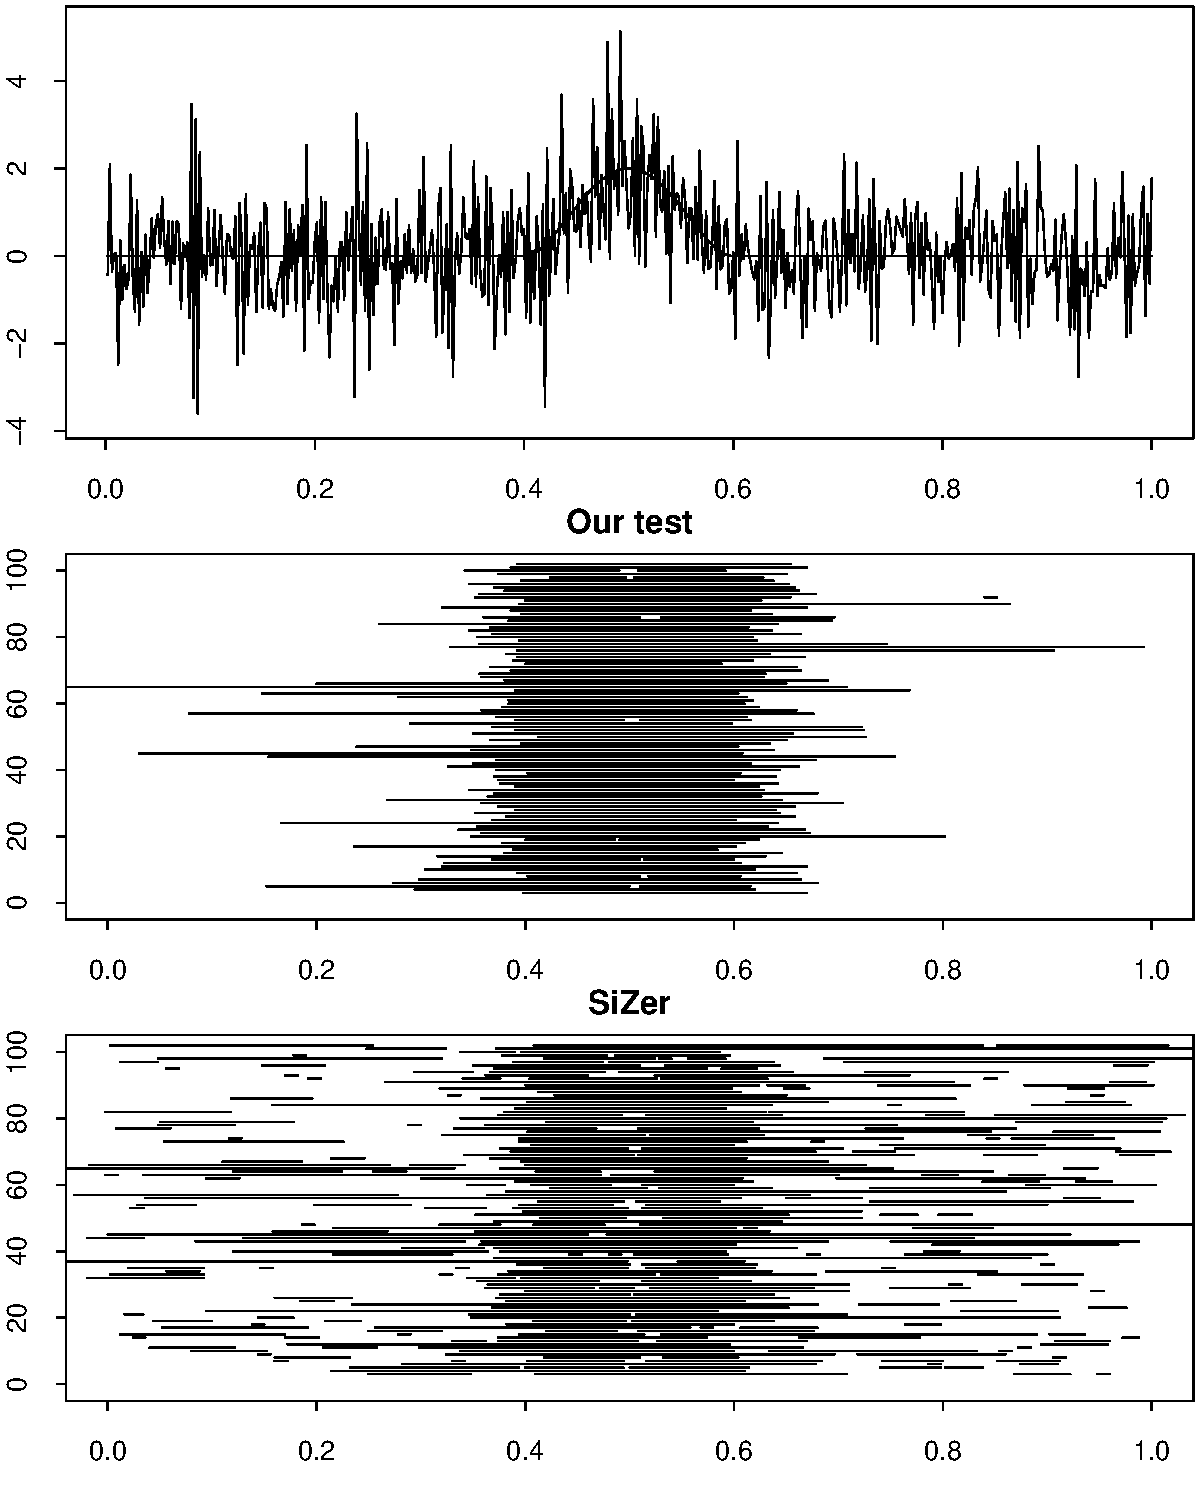
\includegraphics[width=.9\linewidth]{Plots/min_int_with_T_500_a1_-50.pdf}
\caption{$a_1 = -0.5$}
\end{subfigure}
\begin{subfigure}{.5\textwidth}
\centering
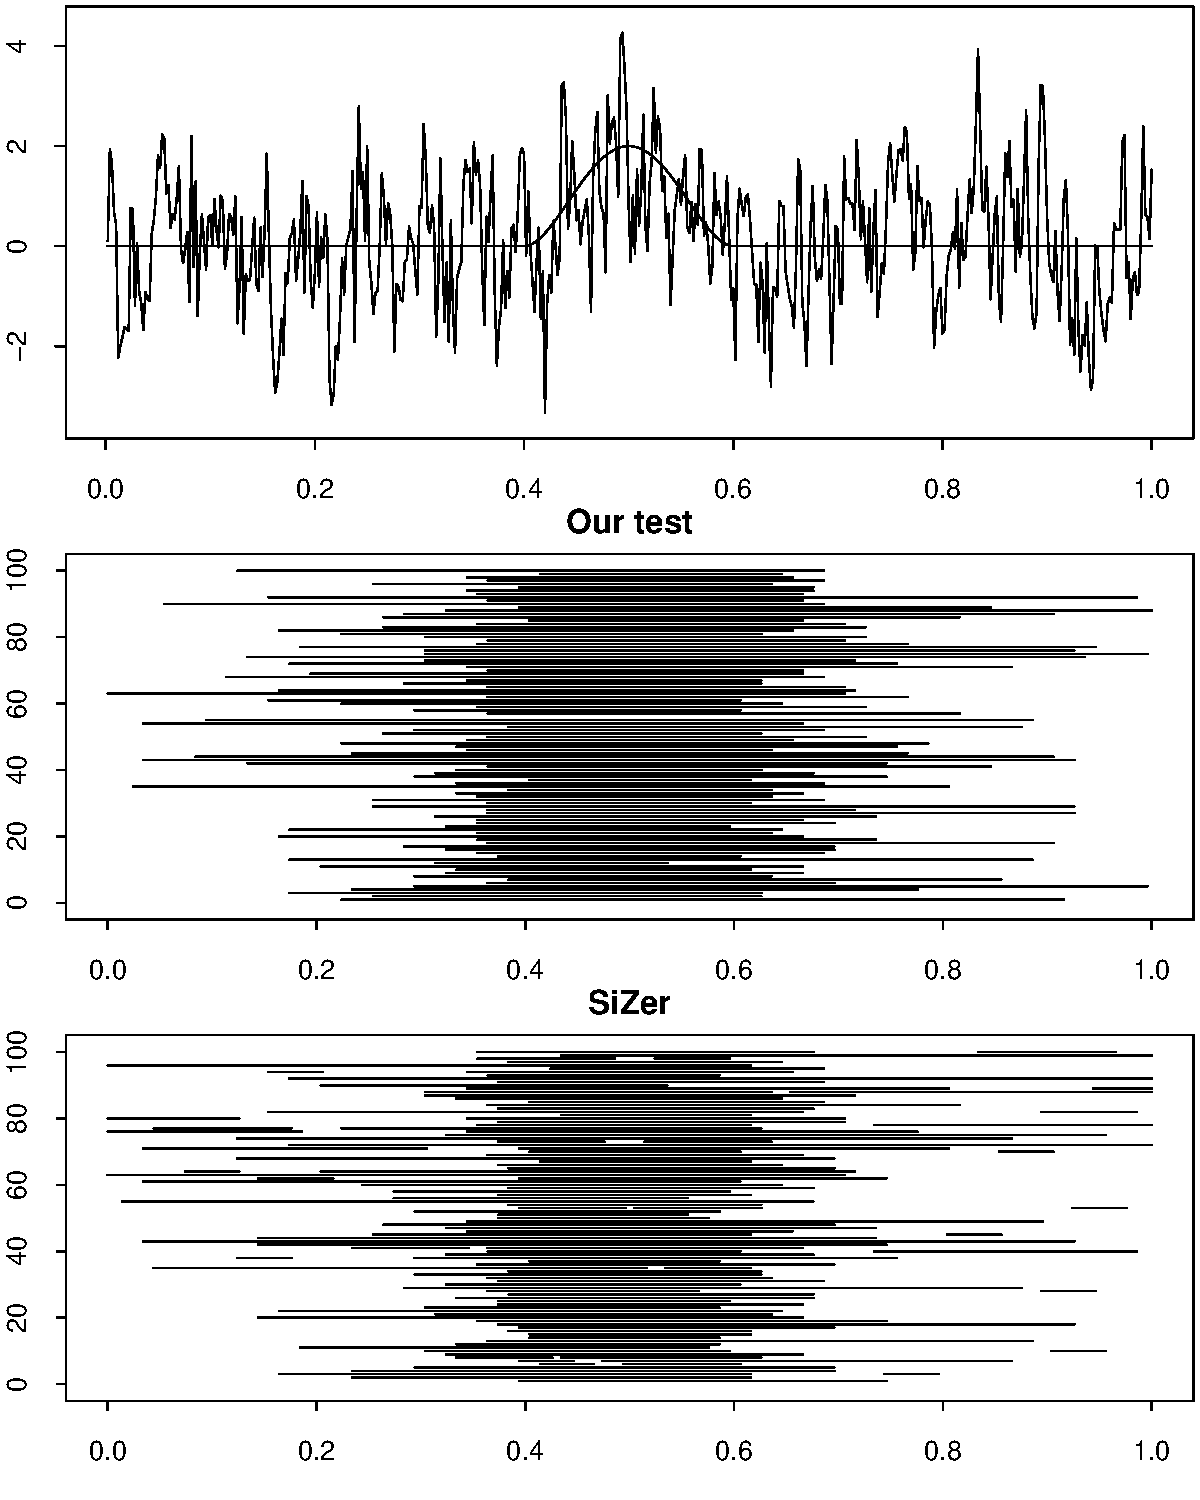
\includegraphics[width=.9\linewidth]{Plots/min_int_with_T_500_a1_50.pdf}
\caption{$a_1 = 0.5$}
\end{subfigure}
\caption{Comparison of the regions $\mathcal{R}_T^\pm$ and $\mathcal{R}_T^{\text{SiZer}}$. Subfigure (a) corresponds to the model setting with the AR parameter $a_1 = -0.5$, subfigure (b) to the setting with $a_1 = 0.5$. The upper panel of each subfigure shows a simulated time series path together with the underlying trend function $m$. The middle panel depicts the regions $\mathcal{R}_T^\pm$ produced by our multiscale test for $100$ simulation runs. The lower panel presents the regions $\mathcal{R}_T^{\text{SiZer}}$ produced by SiZer.}  
\label{fig:comparison_SiZer}
\end{figure}


We consider the same simulation setup as in the first part of the study, only the trend function $m$ is different. We let $m$ be defined as $m(u) = 2 \cdot \ind(u \in [0.4,0.6]) \cdot (1 - 100 \{u-0.5\}^2)^2$, which implies that $\mathcal{R} = [0.4,0.5) \cup (0.5,0.6]$. The function $m$ is plotted in the two upper panels of Figure \ref{fig:comparison_SiZer}. We set the significance level to $\alpha= 0.05$ and the sample size to $T=500$. For each AR parameter $a_1 \in \{ -0.5,0.5 \}$, we simulate $S=100$ samples and compute $\mathcal{R}_T^\pm$ and $\mathcal{R}_T^{\text{SiZer}}$ for each sample. The simulation results are depicted in Figure \ref{fig:comparison_SiZer}, the two subfigures (a) and (b) corresponding to different AR parameters. The upper panel of each subfigure displays the time series path of a representative simulation together with the trend function $m$. The middle panel shows the regions $\mathcal{R}_T^\pm$ produced by our multiscale approach for the $100$ simulation runs: On the $y$-axis, the simulation runs $i$ are enumerated for $1 \le i \le 100$, and the black line at $y$-level $i$ represents $\mathcal{R}_T^\pm$ for the $i$-th simulation. Finally, the lower panel of each subfigure depicts the regions $\mathcal{R}_T^{\text{SiZer}}$ in an analogous way. 


Inspecting Figure \ref{fig:comparison_SiZer}, our multiscale method can be seen to approximate the region $\mathcal{R}$ fairly well in both simulation scenarios under consideration. Especially for the negative AR parameter $a_1 = -0.5$, it performs substantially better than SiZer: For most simulations, $\mathcal{R}_T^\pm$ gives a good approximation to the region $\mathcal{R}$, whereas SiZer identifies regions of decrease/increase all over the unit interval $[0, 1]$. SiZer thus frequently mistakes fluctuations in the time series which are due to the dependence in the error terms for increases/decreases in $m$. For the positive AR parameter $a_1 = 0.5$, the difference in performance is not so pronounced. Nevertheless, also here, SiZer appears to spuriously detect increases/decreases in $m$ outside $\mathcal{R}$ more often than our method. 


To sum up, our multiscale test exhibits good size and power properties in the simulations, and the minimal intervals produced by it identify the time regions where $m$ increases/decreases in a quite reliable way. SiZer performs considerably worse in these respects. Nevertheless, it may still produce informative SiZer plots. % (which is what it is designed for anyway). 
All in all, we would like to regard the two methods as complementary rather than direct competitors. SiZer is an explorative tool which aims to give an overview of the increases/decreases in $m$ by means of a SiZer plot. Our method, in contrast, is tailored to be a rigorous statistical test of the hypothesis $H_0$. In particular, it allows to make rigorous confidence statements about whether and where the trend $m$ increases/decreases. Such statements are not possible with SiZer. 


\subsection{Small sample properties of the long-run variance estimator}\label{subsec-sim-3}


In the final part of the simulation study, we examine the estimators of the AR parameters and the long-run error variance from Section \ref{subsec-error-var-ar}. We simulate data from the model $Y_{t,T} = m(t/T) + \varepsilon_t$, where $\{ \varepsilon_t\}$ is an AR($1$) process of the form $\varepsilon_t = a_1 \varepsilon_{t-1} + \eta_t$. We consider the AR parameters $a_1 \in \{-0.95,-0.75,-0.5,-0.25,0.25,0.5,0.75,0.95\}$ and let $\eta_t$ be i.i.d.\ standard normal innovation terms. For simplicity, $m$ is chosen to be a linear function of the form $m(u) = \beta u$ with $\beta \in \{1,10\}$. The slope parameter $\beta = 1$ corresponds to a moderate trend in the data, whereas the trend becomes quite pronounced for $\beta = 10$. 


\begin{table}[t!]
\centering
\footnotesize{
\caption{Empirical mean and standard deviation of the AR parameter estimators.}\label{tab:AR_parameters}
\newcolumntype{L}{>{\raggedright\arraybackslash}X}
\newcolumntype{C}[1]{>{\hsize=#1\hsize\centering\arraybackslash}X}
\newcolumntype{Z}{>{\centering\arraybackslash}X}
\begin{tabularx}{0.925\textwidth}{LZZZZZ} 
\multicolumn{6}{c}{(a) $\beta = 1$} \\[0.2cm]
\toprule
 & & $\widetilde{a}$ & $\widehat{a}$ & $\widehat{a}_{\text{HvK}}$ & $\widehat{a}_{\text{oracle}}$ \\
\cmidrule[0.4pt]{1-6}
$a = -0.95$ & $T=250$ & 0.000 (0.000) & 0.000 (0.000) & 0.000 (0.000) & 0.000 (0.000) \\
            & $T=500$ & 0.000 (0.000) & 0.000 (0.000) & 0.000 (0.000) & 0.000 (0.000) \\[0.1cm]
$a = -0.75$ & $T=250$ & 0.000 (0.000) & 0.000 (0.000) & 0.000 (0.000) & 0.000 (0.000) \\
            & $T=500$ & 0.000 (0.000) & 0.000 (0.000) & 0.000 (0.000) & 0.000 (0.000) \\[0.1cm]
$a = -0.5$  & $T=250$ & 0.000 (0.000) & 0.000 (0.000) & 0.000 (0.000) & 0.000 (0.000) \\
            & $T=500$ & 0.000 (0.000) & 0.000 (0.000) & 0.000 (0.000) & 0.000 (0.000) \\[0.1cm]
$a = -0.25$ & $T=250$ & 0.000 (0.000) & 0.000 (0.000) & 0.000 (0.000) & 0.000 (0.000) \\
            & $T=500$ & 0.000 (0.000) & 0.000 (0.000) & 0.000 (0.000) & 0.000 (0.000) \\[0.1cm]
$a = 0.25$  & $T=250$ & 0.000 (0.000) & 0.000 (0.000) & 0.000 (0.000) & 0.000 (0.000) \\
            & $T=500$ & 0.000 (0.000) & 0.000 (0.000) & 0.000 (0.000) & 0.000 (0.000) \\[0.1cm]
$a = 0.5$   & $T=250$ & 0.000 (0.000) & 0.000 (0.000) & 0.000 (0.000) & 0.000 (0.000) \\
            & $T=500$ & 0.000 (0.000) & 0.000 (0.000) & 0.000 (0.000) & 0.000 (0.000) \\[0.1cm]
$a = 0.75$  & $T=250$ & 0.000 (0.000) & 0.000 (0.000) & 0.000 (0.000) & 0.000 (0.000) \\
            & $T=500$ & 0.000 (0.000) & 0.000 (0.000) & 0.000 (0.000) & 0.000 (0.000) \\[0.1cm]
$a = 0.95$  & $T=250$ & 0.000 (0.000) & 0.000 (0.000) & 0.000 (0.000) & 0.000 (0.000) \\
            & $T=500$ & 0.000 (0.000) & 0.000 (0.000) & 0.000 (0.000) & 0.000 (0.000) \\
\bottomrule
\end{tabularx}
\vspace{0.25cm}

\begin{tabularx}{0.925\textwidth}{LZZZZZ} 
\multicolumn{6}{c}{(b) $\beta = 10$} \\[0.2cm]
\toprule
 & & $\widetilde{a}$ & $\widehat{a}$ & $\widehat{a}_{\text{HvK}}$ & $\widehat{a}_{\text{oracle}}$ \\
\cmidrule[0.4pt]{1-6}
$a = -0.95$ & $T=250$ & 0.000 (0.000) & 0.000 (0.000) & 0.000 (0.000) & 0.000 (0.000) \\
            & $T=500$ & 0.000 (0.000) & 0.000 (0.000) & 0.000 (0.000) & 0.000 (0.000) \\[0.1cm]
$a = -0.75$ & $T=250$ & 0.000 (0.000) & 0.000 (0.000) & 0.000 (0.000) & 0.000 (0.000) \\
            & $T=500$ & 0.000 (0.000) & 0.000 (0.000) & 0.000 (0.000) & 0.000 (0.000) \\[0.1cm]
$a = -0.5$  & $T=250$ & 0.000 (0.000) & 0.000 (0.000) & 0.000 (0.000) & 0.000 (0.000) \\
            & $T=500$ & 0.000 (0.000) & 0.000 (0.000) & 0.000 (0.000) & 0.000 (0.000) \\[0.1cm]
$a = -0.25$ & $T=250$ & 0.000 (0.000) & 0.000 (0.000) & 0.000 (0.000) & 0.000 (0.000) \\
            & $T=500$ & 0.000 (0.000) & 0.000 (0.000) & 0.000 (0.000) & 0.000 (0.000) \\[0.1cm]
$a = 0.25$  & $T=250$ & 0.000 (0.000) & 0.000 (0.000) & 0.000 (0.000) & 0.000 (0.000) \\
            & $T=500$ & 0.000 (0.000) & 0.000 (0.000) & 0.000 (0.000) & 0.000 (0.000) \\[0.1cm]
$a = 0.5$   & $T=250$ & 0.000 (0.000) & 0.000 (0.000) & 0.000 (0.000) & 0.000 (0.000) \\
            & $T=500$ & 0.000 (0.000) & 0.000 (0.000) & 0.000 (0.000) & 0.000 (0.000) \\[0.1cm]
$a = 0.75$  & $T=250$ & 0.000 (0.000) & 0.000 (0.000) & 0.000 (0.000) & 0.000 (0.000) \\
            & $T=500$ & 0.000 (0.000) & 0.000 (0.000) & 0.000 (0.000) & 0.000 (0.000) \\[0.1cm]
$a = 0.95$  & $T=250$ & 0.000 (0.000) & 0.000 (0.000) & 0.000 (0.000) & 0.000 (0.000) \\
            & $T=500$ & 0.000 (0.000) & 0.000 (0.000) & 0.000 (0.000) & 0.000 (0.000) \\
\bottomrule
\end{tabularx}}
\end{table}


\begin{table}[t!]
\centering
\footnotesize{
\caption{Empirical mean and standard deviation of the long-run variance estimators.}\label{tab:lrv}
\newcolumntype{L}{>{\raggedright\arraybackslash}X}
\newcolumntype{C}[1]{>{\hsize=#1\hsize\centering\arraybackslash}X}
\newcolumntype{Z}{>{\centering\arraybackslash}X}
\begin{tabularx}{0.925\textwidth}{LZZZZZ} 
\multicolumn{6}{c}{(a) $\beta = 1$} \\[0.2cm]
\toprule
 & & $\widetilde{\sigma}^2$ & $\widehat{\sigma}^2$ & $\widehat{\sigma}^2_{\text{HvK}}$ & $\widehat{\sigma}^2_{\text{oracle}}$ \\
\cmidrule[0.4pt]{1-6}
$a = -0.95$ & $T=250$ & 0.000 (0.000) & 0.000 (0.000) & 0.000 (0.000) & 0.000 (0.000) \\
            & $T=500$ & 0.000 (0.000) & 0.000 (0.000) & 0.000 (0.000) & 0.000 (0.000) \\[0.1cm]
$a = -0.75$ & $T=250$ & 0.000 (0.000) & 0.000 (0.000) & 0.000 (0.000) & 0.000 (0.000) \\
            & $T=500$ & 0.000 (0.000) & 0.000 (0.000) & 0.000 (0.000) & 0.000 (0.000) \\[0.1cm]
$a = -0.5$  & $T=250$ & 0.000 (0.000) & 0.000 (0.000) & 0.000 (0.000) & 0.000 (0.000) \\
            & $T=500$ & 0.000 (0.000) & 0.000 (0.000) & 0.000 (0.000) & 0.000 (0.000) \\[0.1cm]
$a = -0.25$ & $T=250$ & 0.000 (0.000) & 0.000 (0.000) & 0.000 (0.000) & 0.000 (0.000) \\
            & $T=500$ & 0.000 (0.000) & 0.000 (0.000) & 0.000 (0.000) & 0.000 (0.000) \\[0.1cm]
$a = 0.25$  & $T=250$ & 0.000 (0.000) & 0.000 (0.000) & 0.000 (0.000) & 0.000 (0.000) \\
            & $T=500$ & 0.000 (0.000) & 0.000 (0.000) & 0.000 (0.000) & 0.000 (0.000) \\[0.1cm]
$a = 0.5$   & $T=250$ & 0.000 (0.000) & 0.000 (0.000) & 0.000 (0.000) & 0.000 (0.000) \\
            & $T=500$ & 0.000 (0.000) & 0.000 (0.000) & 0.000 (0.000) & 0.000 (0.000) \\[0.1cm]
$a = 0.75$  & $T=250$ & 0.000 (0.000) & 0.000 (0.000) & 0.000 (0.000) & 0.000 (0.000) \\
            & $T=500$ & 0.000 (0.000) & 0.000 (0.000) & 0.000 (0.000) & 0.000 (0.000) \\[0.1cm]
$a = 0.95$  & $T=250$ & 0.000 (0.000) & 0.000 (0.000) & 0.000 (0.000) & 0.000 (0.000) \\
            & $T=500$ & 0.000 (0.000) & 0.000 (0.000) & 0.000 (0.000) & 0.000 (0.000) \\
\bottomrule
\end{tabularx}
\vspace{0.25cm}

\begin{tabularx}{0.925\textwidth}{LZZZZZ} 
\multicolumn{6}{c}{(b) $\beta = 10$} \\[0.2cm]
\toprule
 & & $\widetilde{\sigma}^2$ & $\widehat{\sigma}^2$ & $\widehat{\sigma}^2_{\text{HvK}}$ & $\widehat{\sigma}^2_{\text{oracle}}$ \\
\cmidrule[0.4pt]{1-6}
$a = -0.95$ & $T=250$ & 0.000 (0.000) & 0.000 (0.000) & 0.000 (0.000) & 0.000 (0.000) \\
            & $T=500$ & 0.000 (0.000) & 0.000 (0.000) & 0.000 (0.000) & 0.000 (0.000) \\[0.1cm]
$a = -0.75$ & $T=250$ & 0.000 (0.000) & 0.000 (0.000) & 0.000 (0.000) & 0.000 (0.000) \\
            & $T=500$ & 0.000 (0.000) & 0.000 (0.000) & 0.000 (0.000) & 0.000 (0.000) \\[0.1cm]
$a = -0.5$  & $T=250$ & 0.000 (0.000) & 0.000 (0.000) & 0.000 (0.000) & 0.000 (0.000) \\
            & $T=500$ & 0.000 (0.000) & 0.000 (0.000) & 0.000 (0.000) & 0.000 (0.000) \\[0.1cm]
$a = -0.25$ & $T=250$ & 0.000 (0.000) & 0.000 (0.000) & 0.000 (0.000) & 0.000 (0.000) \\
            & $T=500$ & 0.000 (0.000) & 0.000 (0.000) & 0.000 (0.000) & 0.000 (0.000) \\[0.1cm]
$a = 0.25$  & $T=250$ & 0.000 (0.000) & 0.000 (0.000) & 0.000 (0.000) & 0.000 (0.000) \\
            & $T=500$ & 0.000 (0.000) & 0.000 (0.000) & 0.000 (0.000) & 0.000 (0.000) \\[0.1cm]
$a = 0.5$   & $T=250$ & 0.000 (0.000) & 0.000 (0.000) & 0.000 (0.000) & 0.000 (0.000) \\
            & $T=500$ & 0.000 (0.000) & 0.000 (0.000) & 0.000 (0.000) & 0.000 (0.000) \\[0.1cm]
$a = 0.75$  & $T=250$ & 0.000 (0.000) & 0.000 (0.000) & 0.000 (0.000) & 0.000 (0.000) \\
            & $T=500$ & 0.000 (0.000) & 0.000 (0.000) & 0.000 (0.000) & 0.000 (0.000) \\[0.1cm]
$a = 0.95$  & $T=250$ & 0.000 (0.000) & 0.000 (0.000) & 0.000 (0.000) & 0.000 (0.000) \\
            & $T=500$ & 0.000 (0.000) & 0.000 (0.000) & 0.000 (0.000) & 0.000 (0.000) \\
\bottomrule
\end{tabularx}}
\end{table}


For each model specification, we generate $S=1000$ data samples and compute the following quantities for each simulated sample: 
\begin{enumerate}[label=(\roman*),leftmargin=0.9cm]
\item the first step-estimator $\widetilde{a}$ from \eqref{est-AR-FS-av} with the tuning parameters $\underline{q}$ and $\overline{q}$, which nests the estimator $\widetilde{a}_q$ from \eqref{est-AR-FS} as a special case upon setting $\underline{q} = \overline{q} = q$, and the corresponding estimator $\widetilde{\sigma}^2$ of the long-run error variance. 
\item the second-step estimator $\widehat{a}$ from \eqref{est-AR-SS-av} with the tuning parameter $\overline{r}$ and the corresponding long-run variance estimator $\widehat{\sigma}^2$. 
\item the estimators of $a$ and $\sigma^2$ from \cite{Hall2003}, which are denoted by $\widehat{a}_{\text{HvK}}$ and $\widehat{\sigma}^2_{\text{HvK}}$ for ease of reference. The estimator $\widehat{a}_{\text{HvK}}$ is computed as described in Section 2.2 of \cite{Hall2003} and $\widehat{\sigma}^2_{\text{HvK}}$ as defined at the bottom of p.447 in Section 2.3. The estimator $\widehat{a}_{\text{HvK}}$ depends on two tuning parameters which are labelled as $m_1$ and $m_2$ in \cite{Hall2003}. As these are the exact counterparts of $\underline{q}$ and $\overline{q}$, we set $m_1 = \underline{q}$ and $m_2 = \overline{q}$. 
\item oracle estimators $\widehat{a}_{\text{oracle}}$ and $\widehat{\sigma}^2_{\text{oracle}}$ of $a_1$ and $\sigma^2$, which are constructed under the assumption that the error process $\{\varepsilon_t\}$ is observed. For each simulation run, we compute $\widehat{a}_{\text{oracle}}$ as the maximum likelihood estimator of $a_1$ from the time series of simulated error terms $\varepsilon_1,\ldots,\varepsilon_T$. We then calculate the residuals $r_t = \varepsilon_t - \widehat{a}_{\text{oracle}} \, \varepsilon_{t-1}$ and estimate the innovation variance $\nu^2 = \ex[\eta_t^2]$ by $\widehat{\nu}_{\text{oracle}}^2 = (T-1)^{-1} \sum_{t=2}^T r_t^2$. Finally, we set $\widehat{\sigma}^2_{\text{oracle}} = \widehat{\nu}_{\text{oracle}}^2 / (1 - \widehat{a}_{\text{oracle}})^2$. 
\end{enumerate}
Throughout the section, we set $\underline{q}=20$, $\overline{q}=30$ and $\overline{r} = 10$. In order to assess how sensitive our estimators are to the choice of the tuning parameters $\underline{q}$, $\overline{q}$ and $\overline{r}$, we carry out a number of robustness checks, considering a range of different values for $\underline{q}$, $\overline{q}$ and $\overline{r}$. The results are reported in Section ?? in the Supplementary Material. Inspecting the robustness checks, our estimators can be seen to be rather insensitive to the choice of tuning parameters. In particular, we obtain essentially the same results when repeating the simulation exercises of this section for the values of $\underline{q}$, $\overline{q}$ and $\overline{r}$ considered in the Supplementary Material.


\begin{figure}[t!]
\centering
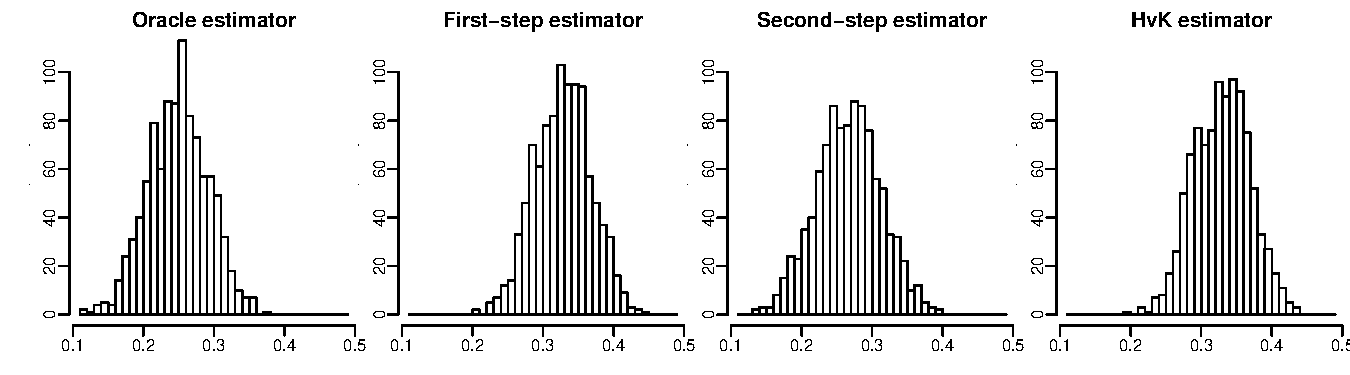
\includegraphics[width=\linewidth]{Plots/variance_histogram_1.pdf}
\caption{Histograms of the simulated values of the estimators $\widetilde{a}$, $\widehat{a}$, $\widehat{a}_{\text{HvK}}$, $\widehat{a}_{\text{oracle}}$ in the simulation scenario with $T=500$, $a_1 = 0.25$ and $\beta = 10$.}\label{fig:hist_AR_scenario1} 
\vspace{0.25cm}

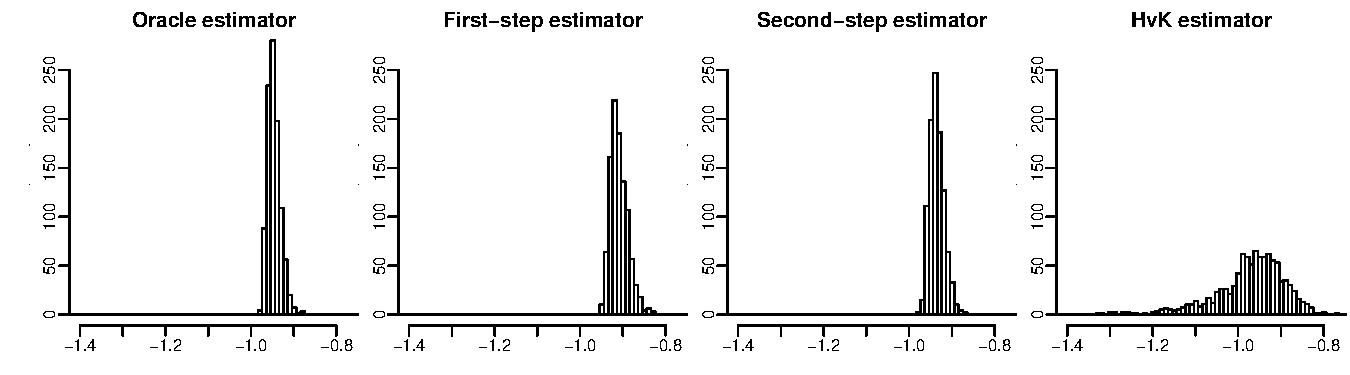
\includegraphics[width=\linewidth]{Plots/variance_histogram_2.pdf}
\caption{Histograms of the simulated values of the estimators $\widetilde{a}$, $\widehat{a}$, $\widehat{a}_{\text{HvK}}$, $\widehat{a}_{\text{oracle}}$ in the simulation scenario with $T=500$, $a_1 = -0.95$ and $\beta = 1$.}\label{fig:hist_AR_scenario2}
\end{figure}


For each estimator $\widetilde{a}$, $\widehat{a}$, $\widehat{a}_{\text{HvK}}$, $\widehat{a}_{\text{oracle}}$ and $\widetilde{\sigma}^2$, $\widehat{\sigma}^2$, $\widehat{\sigma}^2_{\text{HvK}}$, $\widehat{\sigma}^2_{\text{oracle}}$ and for each model specification, the simulation output consists in a vector of length $S=1000$ which contains the $1000$ simulated values of the respective estimator. 
%We denote these vectors by $v(\widetilde{a}_{\text{AV}})$, $v(\widehat{a}_{\text{AV}})$, etc.\ in what follows. 
Tables \ref{tab:AR_parameters} and \ref{tab:lrv} report the empirical mean and standard deviation of these simulated values for each estimator. 
%the vectors $v(\widetilde{a}_{\text{AV}})$, $v(\widehat{a}_{\text{AV}})$, etc.\ 
Moreover, Figures \ref{fig:hist_AR_scenario1} and \ref{fig:hist_AR_scenario2} present histograms of these values for two specific simulation scenarios. The main findings can be summarized as follows: 
\begin{enumerate}[label=(\roman*),leftmargin=0.9cm]

\item The performance of our second-step estimators $\widehat{a}$ and $\widehat{\sigma}^2$ is fairly close to that of the oracle estimators $\widehat{a}_{\text{oracle}}$ and $\widehat{\sigma}^2_{\text{oracle}}$ in all of the considered simulation scenarios. In particular, the mean values and standard deviations in Tables \ref{tab:AR_parameters} and \ref{tab:lrv} are quite similar for our estimators and the corresponding oracles. 

\item In the simulation scenarios with a moderate trend ($\beta = 1$), the first-step estimators $\widetilde{a}$ and $\widetilde{\sigma}^2$ produce results very similar to those of the second-step estimators $\widehat{a}$ and $\widehat{\sigma}^2$. However, in the scenarios with a pronounced trend ($\beta = 10$), the first-step estimators are strongly biased. The reason is that the trend is not eliminated appropriately by them. The second-step estimators substantially reduce this bias. This point is nicely illustrated by Figure \ref{fig:hist_AR_scenario1} which shows histograms of the simulated values of the estimators $\widetilde{a}$, $\widehat{a}$, $\widehat{a}_{\text{HvK}}$, $\widehat{a}_{\text{oracle}}$ in the scenario with $T=500$, $a_1=0.25$ and $\beta = 10$. As one can see, the histogram produced by our second-step estimator $\widehat{a}$ is nicely centred around the true value $a_1 = 0.25$, whereas those of the estimators $\widetilde{a}$ and $\widehat{a}_{\text{HvK}}$ are strongly biased upwards. 

\item The estimators $\widehat{a}_{\text{HvK}}$ and $\widehat{\sigma}^2_{\text{HvK}}$ of \cite{Hall2003} exhibit a similar performance as our first-step estimators $\widetilde{a}$ and $\widetilde{\sigma}^2$ as long as the AR parameter $a_1$ is not too close to $-1$. For strongly negative values of $a_1$ (in particular for $a_1 = -0.75$ and $a_1 = -0.95$), the estimators perform much worse than ours. This is already indicated by the extremely large variances of the estimators $\widehat{a}_{\text{HvK}}$ and $\widehat{\sigma}^2_{\text{HvK}}$ in Tables \ref{tab:AR_parameters} and \ref{tab:lrv} in the scenarios with $a_1 \in \{-0.75,-0.95\}$. Figure \ref{fig:hist_AR_scenario1} gives some further insights into what is happening here. It presents the histograms of the simulated values of $\widetilde{a}$, $\widehat{a}$, $\widehat{a}_{\text{HvK}}$, $\widehat{a}_{\text{oracle}}$ in the scenario with $T=500$, $a_1=-0.95$ and $\beta = 1$. As can be seen, the estimator $\widehat{a}_{\text{HvK}}$ does not obey the causality restriction $|a_1| \le 1$ but frequently takes values smaller than $-1$. This results in a very large spread of the histogram and thus in a disastrous performance of the estimator. Our estimators $\widetilde{a}$ and $\widehat{a}$, in contrast, exhibit a stable behaviour in this case.
\end{enumerate}



\section{Application}\label{sec-data}


The analysis of time trends in long temperature records is an important task in climatology. Information on the shape of the trend is needed in order to better understand long-term climate variability. The Central England temperature record is the longest instrumental temperature time series in the world. It is a valuable asset for analysing climate variability over the last few hundred years. The data is publicly available on the webpage of the UK Met Office. A detailed description of the data can be found in \cite{Parker1992}. For our analysis, we use the dataset of yearly mean temperatures which consists of $T=359$ observations covering the years from $1659$ to $2017$. We assume that the data follow the nonparametric trend model $Y_{t,T} = m(t/T) + \varepsilon_t$, where $m$ is the unknown time trend of interest. The error process $\{ \varepsilon_t \}$ is supposed to have the AR($p$) structure $\varepsilon_t = \sum_{j=1}^p a_j \varepsilon_{t-j} + \eta_t$, where $\eta_t$ are i.i.d.\ innovations with mean $0$ and variance $\nu^2$. As pointed out in \cite{Mudelsee2010} among others, this is the most widely used error model for discrete climate time series. We select the AR order $p$ by minimizing an FPE criterion, which yields the AR $p=2$. We then estimate the parameters $a_1$, $a_2$ and $\nu^2$ as described in Section \ref{subsec-error-var-ar} which yields the estimates $\widehat{a}_1 \approx ??$, $\widehat{a}_2 \approx ??$ and $\widehat{\nu}^2 \approx ??$.


\begin{figure}[t]
\centering
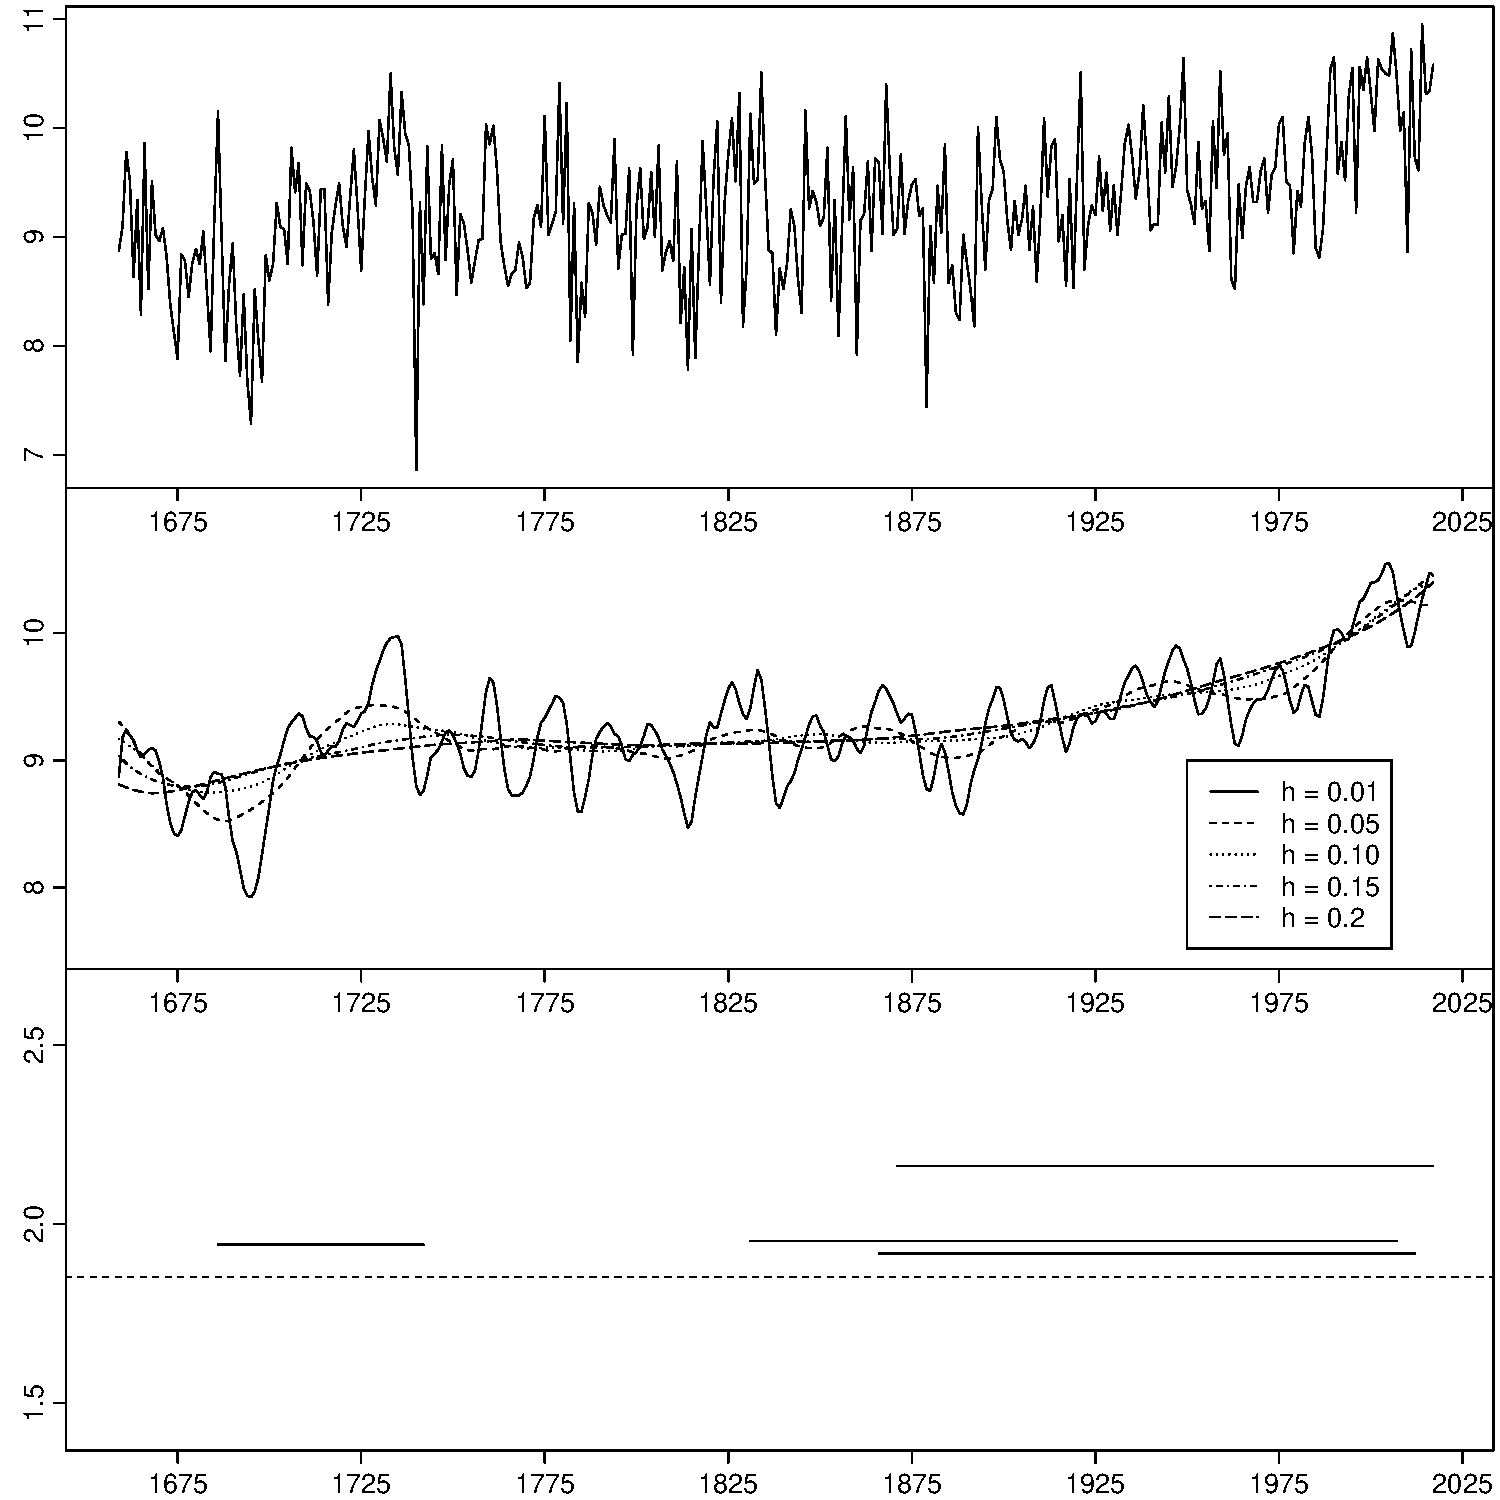
\includegraphics[width=0.8\textwidth]{Plots/temperature_L1_20_L2_30.pdf}
\caption{Summary of the application results for Section \ref{sec-data}. The upper panel shows the Central England mean temperature time series. The middle panel depicts local linear kernel estimates of the time trend for a number of different bandwidths $h$. The lower panel presents the minimal intervals in the set $\Pi_T^+$ produced by the multiscale test. These are $[??,??]$, $[??,??]$, $[??,??]$ and $[??,??]$.}\label{plot-results-app1}
\end{figure}


With the help of our multiscale method from Section \ref{sec-method}, we test the null hypothesis $H_0$ that $m$ is constant on all intervals $[u-h,u+h]$ with $(u,h) \in \mathcal{G}_T$, where we use the grid $\mathcal{G}_T$ defined in \eqref{grid-sim-app}. To do so, we set the significance level to $\alpha = 0.05$ and implement the test in exactly the same way as in the simulations of Section \ref{sec-sim}. The results are presented in Figure \ref{plot-results-app1}. The upper panel shows the raw temperature time series, whereas the middle panel depicts local linear kernel estimates of the trend $m$ for different bandwidths $h$. As one can see, the shape of the estimated time trend strongly differs with the chosen bandwidth. When the bandwidth is small, there are many local increases and decreases in the estimated trend. When the bandwidth is large, most of these local variations get smoothed out. Hence, by themselves, the nonparametric fits do not give much information on whether the trend $m$ is increasing or decreasing in certain time regions. 


Our multiscale test provides this kind of information, which is summarized in the lower panel of Figure \ref{plot-results-app1}. The plot depicts the minimal intervals contained in the set $\Pi_T^+$ which is defined in Section \ref{subsec-method-theo}. The set of intervals $\Pi_T^-$ is empty in the present case. The height at which a minimal interval $I_{u,h} = [u-h,u+h] \in \Pi_t^+$ is plotted indicates the value of the corresponding (additively corrected) test statistic $\widehat{\psi}_T(u,h) / \widehat{\sigma} - \lambda(h)$. The dashed line specifies the critical value $q_T(\alpha)$, where $\alpha = 0.05$ as already mentioned above. According to Proposition \ref{prop-test-3}, we can make the following simultaneous confidence statement about the collection of minimal intervals in $\Pi_T^+$. We can claim, with confidence of about $95\%$, that the trend function $m$ has some increase on each minimal interval. More specifically, we can claim with this confidence that there has been some upward movement in the trend both in the period from around $1680$ to $1740$ and in the period from about $1880$ onwards. Hence, our test in particular provides evidence that there has been some warming trend in the period over approximately the last $140$ years. On the other hand, as the set $\Pi_T^-$ is empty, there is no evidence of any downward movement of the trend.  



\bibliographystyle{ims}
{\small
\setlength{\bibsep}{0.45em}
\bibliography{bibliography}}



\end{document}
